\documentclass[12pt,a4paper]{book}

% ========================================
% PREAMBLE for Probability and Statistics (Classical Grayscale)
% ========================================

% --- Basics ---
\usepackage[utf8]{inputenc}
\usepackage[T1]{fontenc}
\usepackage{textcomp}
\usepackage{graphicx}
\usepackage{float}
\usepackage{booktabs}
\usepackage[shortlabels]{enumitem}
\usepackage{emptypage}
\usepackage{subcaption}
\usepackage{multicol}
\usepackage[usenames,dvipsnames]{xcolor}
\setlength{\headheight}{14.5pt}

% --- Math Packages ---
\usepackage{amsmath, amsfonts, mathtools, amsthm, amssymb}
\usepackage{mathrsfs}
\usepackage{cancel}
\usepackage{bm}
\usepackage[cal=boondoxo]{mathalfa}
\usepackage{systeme}
\usepackage{stmaryrd}

% --- Math Commands ---
\newcommand\N{\mathbb{N}}
\newcommand\R{\mathbb{R}}
\newcommand\Z{\mathbb{Z}}
\renewcommand\O{\emptyset}
\newcommand\Q{\mathbb{Q}}
\newcommand\C{\mathbb{C}}
\newcommand{\samplespace}{\mathcal{S}}
\DeclareMathOperator{\sgn}{sgn}
\let\implies\Rightarrow
\let\impliedby\Leftarrow
\let\iff\Leftrightarrow
\let\epsilon\varepsilon
\newcommand\contra{\scalebox{1.1}{$\lightning$}}
\newcommand\mat[1]{\mathbf{#1}}

% --- Correction Commands ---
\definecolor{correct}{HTML}{555555} % subtle gray
\newcommand\correct[2]{\ensuremath{\:}{\color{red}{#1}}\ensuremath{\to}{\color{black!70}{#2}}\ensuremath{\:}}
\newcommand\green[1]{{\color{correct}{#1}}}

% --- Utilities ---
\usepackage{xifthen}
\newcommand\hr{\noindent\rule[0.5ex]{\linewidth}{0.5pt}}
\newcommand\hide[1]{}

% --- SI Units ---
\usepackage{siunitx}
\sisetup{locale=FR}

% --- TikZ ---
\usepackage{tikz}
\usepackage{tikz-cd}
\usetikzlibrary{intersections, angles, quotes, calc, positioning, arrows.meta, shapes, trees}
\usepackage{pgfplots}
\pgfplotsset{compat=1.13}
\tikzset{
    force/.style={thick, {Circle[length=2pt]}-Stealth, shorten <=-1pt, draw=black!70}
}

% --- Page Layout ---
\usepackage[top=3cm,bottom=3cm,inner=3cm,outer=2.5cm]{geometry}
\setlength{\headheight}{13.6pt}

% --- Theorem Styles ---
\usepackage{thmtools}
\usepackage[framemethod=TikZ]{mdframed}
\mdfsetup{skipabove=1em, skipbelow=0em, innertopmargin=5pt, innerbottommargin=6pt}

\theoremstyle{definition}

% --- Grayscale Theorem Styles ---
\declaretheoremstyle[
    headfont=\bfseries\sffamily,
    bodyfont=\normalfont,
    mdframed={
        linewidth=2pt, rightline=false, topline=false, bottomline=false,
        linecolor=black!50, backgroundcolor=black!5
    }
]{thmgreenbox}

\declaretheoremstyle[
    headfont=\bfseries\sffamily,
    bodyfont=\normalfont,
    mdframed={
        linewidth=2pt, rightline=false, topline=false, bottomline=false,
        linecolor=black!50, backgroundcolor=black!10
    }
]{thmbluebox}

\declaretheoremstyle[
    headfont=\bfseries\sffamily,
    bodyfont=\normalfont,
    mdframed={
        linewidth=2pt, rightline=false, topline=false, bottomline=false,
        linecolor=black!50
    }
]{thmblueline}

\declaretheoremstyle[
    headfont=\bfseries\sffamily,
    bodyfont=\normalfont,
    mdframed={
        linewidth=2pt, rightline=false, topline=false, bottomline=false,
        linecolor=black!50, backgroundcolor=black!10
    }
]{thmredbox}

\declaretheoremstyle[
    headfont=\bfseries\sffamily,
    bodyfont=\normalfont,
    numbered=no,
    mdframed={
        linewidth=2pt, rightline=false, topline=false, bottomline=false,
        linecolor=black!50, backgroundcolor=black!2
    },
    qed=\qedsymbol
]{thmproofbox}

\declaretheoremstyle[
    headfont=\bfseries\sffamily,
    bodyfont=\normalfont,
    numbered=no,
    mdframed={
        linewidth=2pt, rightline=false, topline=false, bottomline=false,
        linecolor=black!50, backgroundcolor=black!2
    },
]{thmexplanationbox}

% --- Theorem Declarations ---
\declaretheorem[style=thmsolutionbox, name=Solution]{solution}
\declaretheorem[style=thmgreenbox, name=Definition]{definition}
\declaretheorem[style=thmbluebox, numbered=no, name=Example]{eg}
\declaretheorem[style=thmbluebox, name=Exercise]{exercise}
\declaretheorem[style=thmredbox, name=Proposition]{prop}
\declaretheorem[style=thmredbox, name=Theorem]{theorem}
\declaretheorem[style=thmredbox, name=Lemma]{lemma}
\declaretheorem[style=thmredbox, numbered=no, name=Corollary]{corollary}
\declaretheorem[style=thmproofbox, name=Proof]{replacementproof}
\renewenvironment{proof}[1][\proofname]{\vspace{-10pt}\begin{replacementproof}}{\end{replacementproof}}
\declaretheorem[style=thmexplanationbox, name=Explanation]{explanation}
\declaretheorem[style=thmblueline, numbered=no, name=Remark]{remark}
\declaretheorem[style=thmblueline, numbered=no, name=Note]{note}

\newtheorem*{notation}{Notation}
\newtheorem*{previouslyseen}{As previously seen}
\newtheorem*{problem}{Problem}
\newtheorem*{observe}{Observe}
\newtheorem*{property}{Property}
\newtheorem*{intuition}{Intuition}

% --- Lecture & Exercise Commands ---
\makeatletter
\newlist{subtasks}{enumerate}{1}
\setlist[subtasks,1]{label=\alph*)}
\def\@lesson{}%
\newcommand{\lesson}[3]{%
    \ifthenelse{\isempty{#3}}{%
        \def\@lesson{Lecture #1}%
    }{%
        \def\@lesson{Lecture #1: #3}%
    }%
    \subsection*{\@lesson}%
    \marginpar{\small\textsf{\mbox{#2}}}%
}
\makeatother

% --- Headers and Footers ---
\usepackage{fancyhdr}
\pagestyle{fancy}
\fancyhead{}
\fancyhead[RO,LE]{MTH 3301}
\fancyfoot[LE,RO]{\thepage}
\fancyfoot[C]{\leftmark}
\renewcommand{\headrulewidth}{0.4pt}

% --- Notes ---
\usepackage{tcolorbox}
\tcbuselibrary{breakable}
\newenvironment{verbetering}{\begin{tcolorbox}[
    arc=0mm, colback=white, colframe=black!50,
    title=Remark, fonttitle=\sffamily, breakable
]}{\end{tcolorbox}}

\newenvironment{noot}[1]{\begin{tcolorbox}[
    arc=0mm, colback=white, colframe=black!30,
    title=#1, fonttitle=\sffamily, breakable
]}{\end{tcolorbox}}

% --- Figure Support ---
\usepackage{import}
\usepackage{pdfpages}
\usepackage{transparent}
\newcommand{\incfig}[1]{%
    \def\svgwidth{\columnwidth}
    \import{./figures/}{#1.pdf_tex}
}
\pdfsuppresswarningpagegroup=1

% --- Hyperlinks ---
\usepackage{hyperref}
\hypersetup{
    colorlinks=false,
    pdfborder={0 0 0}
}

\setlength{\headheight}{15pt}
\addtolength{\topmargin}{-2pt}

\title{\textbf{Probability and Statistics}}
\author{H.B}
\date{\today}

\begin{document}

\begin{titlepage}
    \centering
    \vspace*{2.5cm}
    {\Huge\bfseries Probability and Statistics\par}
    \vspace{1cm}
    \hrule
    \vspace{0.5cm}
    {\LARGE \textit{Lecture Notes}\par}
    \vspace{0.5cm}
    \hrule
    \vspace{2cm}
    {\Large \textsc{Hamza Berahma}\par}
    \vspace{0.5cm}
    {\large Student\par}
    \vfill
    {\large \today\par}
    \vspace{1cm}
\end{titlepage}

\cleardoublepage
\thispagestyle{empty}
\vspace*{6cm}
\begin{center}
    \emph{For} \\[0.5cm]
    \rule{1.5cm}{0.4pt}\\[0.5cm]
    \emph{my idea of beautiful}
\end{center}
\vfill

\frontmatter
\tableofcontents

\mainmatter
\chapter{Foundations of Probability}
\label{ch:foundations}

% --- Section: Intuition ---
\section{Probability and Intuition}

Sometimes our intuition misleads us. To be more accurate, we need to recognize that intuition can be wrong for mainly two reasons:

\begin{enumerate}
    \item Misunderstanding the terminology of the problem.
    \item Biases from past experiences.
\end{enumerate}

\begin{intuition}
Intuition about probability often fails because our minds rely on past experience or oversimplified reasoning. Being aware of this can help us approach problems more carefully.
\end{intuition}

\begin{problem}
Consider the following statements. Decide whether they are true or false, and explain why.
\end{problem}

\begin{eg}[Fair Coin Toss]
\textbf{Statement:} When we toss a fair coin, the chance of heads is $\frac{1}{2}$ and the chance of tails is $\frac{1}{2}$.  

\textbf{Answer:} True. This is the definition of a fair coin.
\end{eg}

\begin{eg}[Possible Outcomes]
\textbf{Statement:} When we toss a coin, there are 2 possible outcomes: H or T.  

\textbf{Answer:} Mostly true, but it depends on the experiment's definition. What if the coin lands on its edge? We typically simplify the model to include only Heads and Tails.
\end{eg}

\begin{eg}[Mean vs. Median]
\textbf{Statement:} We have a set of 1000 numbers. Their average is $A$. Half the numbers are $\leq A$, and half are $> A$.  

\textbf{Answer:} False. This describes the \textbf{median}, not the \textbf{average} (mean). Consider the set $\{1, 2, 97\}$. The average is $A=33.3$, but two-thirds of the numbers are less than $A$.
\end{eg}

\begin{eg}[Random Number Probability]
\textbf{Statement:} I will randomly pick a number from $\{1, 2, 3, 4\}$. What is $P(1)$?  

\textbf{Answer:} It is $\frac{1}{4}$, but only if "randomly" implies that each outcome is equally likely (a uniform distribution). The term "random" alone is not sufficient.
\end{eg}

\begin{eg}[Average Number of Legs]
\textbf{Statement:} What are the chances that the next person who walks into this room has more than the average number of legs?  

\textbf{Answer:} Extremely high (close to 100\%). The vast majority of people have two legs. A very small number of people have one or zero legs. The average number of legs for a human population will be slightly less than 2 (e.g., 1.999...). Therefore, almost everyone has more than the average.
\end{eg}

\begin{remark}
Always clarify definitions and assumptions in probability problems. \\
Words like "random" or "average" can be misleading if interpreted naively.
\end{remark}
% --- Section: Experiments and Sample Spaces ---
\section{Random Experiments and Sample Spaces}

To formalize probability, we begin with a few core definitions.

\begin{definition}[Random Experiment]
A well-defined procedure that results in an uncertain outcome.
\end{definition}

\begin{definition}[Outcome]
A single result of a random experiment.
\end{definition}

\begin{definition}[Sample Space]
The set of all possible outcomes of a random experiment, denoted $S$.
\end{definition}

\begin{definition}[Trial]
Each attempt or performance of a random experiment is called a trial.
\end{definition}

\begin{definition}[Event]
Any subset of the sample space ($A \subseteq S$). An event is a set of outcomes.
\end{definition}

\begin{remark}
The most critical step in solving a probability problem is often defining the sample space correctly. A poorly defined sample space can lead to incorrect probability calculations.
\end{remark}

\begin{eg}[Examples of Sample Spaces]
Here are several random experiments and their corresponding sample spaces:

\begin{description}
    \item[$E_1$:] Roll a fair die and record the top face. \\
    $S_1 = \{1, 2, 3, 4, 5, 6\}$

    \item[$E_2$:] Toss a coin twice and record the sequence of outcomes. \\
    $S_2 = \{HH, HT, TH, TT\}$

    \item[$E_3$:] Toss a die twice and record the sum of the faces. \\
    $S_3 = \{2, 3, \dots, 12\}$

    \item[$E_4$:] Toss a 3-sided die twice and record the ordered pair of results. \\
    $S_4 = \{(i,j) : i,j \in \{1,2,3\}\} = \{(1,1), (1,2), (1,3), (2,1), \dots, (3,3)\}$

    \item[$E_5$:] Toss a 3-sided die twice and record the set of results (order ignored). \\
    $S_5 = \{\{i,j\} : i,j \in \{1,2,3\}\} = \{\{1,1\}, \{1,2\}, \{1,3\}, \{2,2\}, \{2,3\}, \{3,3\}\}$

    \item[$E_6$:] Toss a coin until the first head appears, recording the number of tosses. \\
    $S_6 = \{1, 2, 3, \dots \} = \mathbb{N}^+$

    \item[$E_7$:] Pick a random English word and record its number of letters. \\
    $S_7 = \{1, 2, 3, \dots \}$
\end{description}
\end{eg}
% --- Section: Probability Measures ---
\section{Probability Measures}

A probability measure (or probability distribution) is a function that assigns a likelihood to each event.

\begin{definition}[Probability Measure]
A probability measure is a function 
\[
P: \mathcal{P}(S) \to [0,1]
\] 
that maps events in the sample space $S$ to a real number between 0 and 1. It must satisfy the following three axioms:
\begin{enumerate}
    \item \textbf{Non-negativity:} For any event $A \subseteq S$, $P(A) \geq 0$.
    \item \textbf{Normalization:} The probability of the entire sample space is 1, i.e., $P(S) = 1$.
    \item \textbf{Additivity:} For any finite collection of pairwise disjoint events. \\ 
    $$A_1, A_2, \dots, A_n$$ (meaning $A_i \cap A_j = \emptyset$ for $i \neq j$), \\ 
    the probability of their union is the sum of their individual probabilities:
    \[
        P\left(\bigcup_{i=1}^{n} A_i\right) = \sum_{i=1}^{n} P(A_i).
    \]
\end{enumerate}
\end{definition}

\begin{remark}
Intuitively, a probability measure quantifies how likely an event is to occur. The axioms ensure probabilities are consistent: they cannot be negative, the total probability is 1, and disjoint events’ probabilities add up.
\end{remark}
% --- Section: Computing Probabilities ---
\section{Computing Probabilities}

Let's apply the concepts of probability measures to compute probabilities in various scenarios.

\begin{eg}[Fair 12-sided Die]
Throw a fair 12-sided die. The sample space is $S = \{1, 2, \dots, 12\}$. Each outcome has probability $\frac{1}{12}$. Let $E$ be the event of rolling an even number and $F$ be the event of rolling a number $\le 4$:
\[
    E = \{2, 4, 6, 8, 10, 12\}, \quad F = \{1, 2, 3, 4\}.
\]
The probabilities are:
\begin{itemize}
    \item $P(E) = \frac{|E|}{|S|} = \frac{6}{12} = \frac{1}{2}$
    \item $P(F) = \frac{|F|}{|S|} = \frac{4}{12} = \frac{1}{3}$
    \item $P(E \cap F) = P(\{2,4\}) = \frac{2}{12} = \frac{1}{6}$
    \item $P(F^c) = 1 - P(F) = 1 - \frac{1}{3} = \frac{2}{3}$
\end{itemize}
\end{eg}

\begin{eg}[Sum of Two Dice]
Throw a fair 6-sided die twice and record the sum. The sample space of ordered pairs is $S' = \{(i,j) : i,j \in \{1,\dots,6\}\}$, so $|S'| = 36$. The sample space for the sum is $S = \{2, 3, \dots, 12\}$. Outcomes in $S$ are not equally likely. Let $E$ be the event that the sum is even.
\[
P(\text{Sum}=2) = \frac{1}{36}, \quad 
P(\text{Sum}=3) = \frac{2}{36}, \quad 
P(\text{Sum}=4) = \frac{3}{36}.
\]

\begin{center}
\begin{tabular}{lcccccc}
\toprule
Sum & 2 & 4 & 6 & 8 & 10 & 12 \\
\midrule
\# Ways & 1 & 3 & 5 & 5 & 3 & 1 \\
\bottomrule
\end{tabular}
\end{center}

So, 
\[
P(E) = \frac{1+3+5+5+3+1}{36} = \frac{18}{36} = \frac{1}{2}.
\]
\end{eg}

\begin{eg}[Weighted Die]
Consider a 5-sided die where $P(k) = c \cdot k$. Using normalization $\sum_{k=1}^{5} P(k) = 1$:
\[
c(1+2+3+4+5) = 15c = 1 \implies c = \frac{1}{15}.
\]
Then $P(k) = \frac{k}{15}$. The probability of rolling an even face is
\[
P(\text{even}) = P(\{2,4\}) = \frac{2}{15} + \frac{4}{15} = \frac{6}{15} = \frac{2}{5}.
\]
\end{eg}

\begin{eg}[Permutations]
Consider all permutations of $\{1,2,3\}$ with equal probability. Let $E$ be "starts with 1" and $F$ be "2 comes before 3":
\[
E = \{123, 132\} \implies P(E) = \frac{2}{6} = \frac{1}{3}, \quad 
F = \{123, 213, 231\} \implies P(F) = \frac{3}{6} = \frac{1}{2}.
\]
\end{eg}

\begin{eg}[Weighted Permutations]
Consider permutations of $\{1,2,3,4\}$. Let $P(abcd) \propto a$, the first element. Sum of weights: \\ 
$6(1)+6(2)+6(3)+6(4) = 60 \implies P(x) = \frac{a}{60}$.  

Let $E = \{abcd \in S_4 \mid a<b \text{ and } c<d\} = \{1234, 1324, 1423, 2314, 2413, 3412\}$. Then
\[
P(E) = \frac{1+1+1+2+2+3}{60} = \frac{10}{60} = \frac{1}{6}.
\]
\end{eg}

\begin{remark}
Weighted probabilities allow modeling biased or non-uniform scenarios. Always normalize probabilities to ensure the total sum equals 1.
\end{remark}
% --- Section: Conditional Probability ---
\section{Conditional Probability}

Conditional probability measures the likelihood of an event occurring given that another event has already occurred. It is a fundamental concept that allows us to update our beliefs in light of new evidence.

\begin{definition}[Conditional Probability]
Given two events $A$ and $B$ from a sample space $S$, with $P(B) > 0$, the \textbf{conditional probability of $A$ given $B$} is defined as:
\[
    P(A|B) = \frac{P(A \cap B)}{P(B)}.
\]
This formula re-scales the probability of the intersection of $A$ and $B$ by the probability of the given event, $B$. In essence, we are treating $B$ as our new, smaller sample space.
\end{definition}

\begin{eg}[Medical Testing]
Consider a medical test for a disease. Let $S$ be the event that a person has the disease, and $\bar{S}$ the event they do not. Let \texttt{pos} and \texttt{neg} denote positive and negative test results, respectively.

We are given:
\begin{itemize}
    \item The probability of having the disease (prevalence): $P(S) = 0.20$ ($P(\bar{S}) = 0.80$).
    \item Probability of a positive test if the patient has the disease (sensitivity): $P(\text{pos}|S) = 0.97$.
    \item Probability of a negative test if the patient does not have the disease (specificity): $P(\text{neg}|\bar{S}) = 0.90$.
\end{itemize}

From these, we deduce:
\begin{itemize}
    \item False Negative Rate: $P(\text{neg}|S) = 1 - 0.97 = 0.03$.
    \item False Positive Rate: $P(\text{pos}|\bar{S}) = 1 - 0.90 = 0.10$.
\end{itemize}

\paragraph{Step 1: Compute Joint Probabilities}
Using the multiplication rule $P(A \cap B) = P(B) P(A|B)$:
\begin{align*}
    P(S \cap \text{pos}) &= 0.20 \times 0.97 = 0.194, \\
    P(S \cap \text{neg}) &= 0.20 \times 0.03 = 0.006, \\
    P(\bar{S} \cap \text{pos}) &= 0.80 \times 0.10 = 0.080, \\
    P(\bar{S} \cap \text{neg}) &= 0.80 \times 0.90 = 0.720.
\end{align*}

\begin{figure}[H]
    \centering
    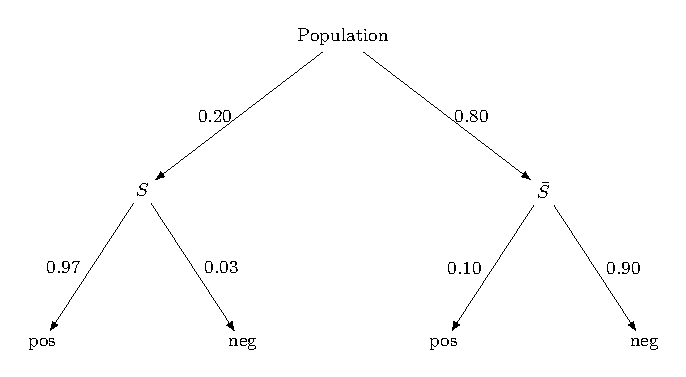
\includegraphics[width=0.7\textwidth]{figures/tree_medicalTesting.pdf}
    \caption{Tree diagram illustrating the relationships between disease status and test results.}
    \label{fig:tree_medical_testing}
\end{figure}

\paragraph{Step 2: Compute the Marginal Probability of a Positive Test}
\[
    P(\text{pos}) = P(S \cap \text{pos}) + P(\bar{S} \cap \text{pos}) = 0.194 + 0.080 = 0.274.
\]

\paragraph{Step 3: Compute the Posterior Probability}
\[
    P(S|\text{pos}) = \frac{P(S \cap \text{pos})}{P(\text{pos})} = \frac{0.194}{0.274} \approx 0.708.
\]

\begin{intuition}[Understanding Bayes' Theorem]
Even with a highly accurate test, a positive result does not guarantee the presence of the disease. This is because the overall prevalence of the disease in the population affects the probability. Bayes' theorem allows us to "update" our belief by combining the test's accuracy with prior information (prevalence).
\end{intuition}
\end{eg}


\begin{eg}[Blood Type Distribution]
The joint probability distribution \( P(\text{Type} \cap \text{Category}) \) for individuals classified by blood type and category (P, Q, R, S, T) is given in Table~\ref{tab:bloodtype}.

\begin{table}[H]
    \centering
    \begin{tabular}{l|ccccc}
        \toprule
        \textbf{Blood Type} & \textbf{P} & \textbf{Q} & \textbf{R} & \textbf{S} & \textbf{T} \\
        \midrule
        A  & 0.30 & 0.40 & 0.20 & 0.45 & 0.20 \\
        B  & 0.30 & 0.30 & 0.10 & 0.45 & 0.20 \\
        AB & 0.20 & 0.10 & 0.40 & 0.05 & 0.30 \\
        O  & 0.20 & 0.20 & 0.30 & 0.05 & 0.30 \\
        \bottomrule
    \end{tabular}
    \caption{Rescaled joint distribution where each category column sums to 1.}
    \label{tab:bloodtype}
\end{table}

\paragraph{(a) Probability of blood type A given category T}
\[
P(A \mid T) = \frac{P(A \cap T)}{P(T)} = \frac{0.20}{1.00} = 0.20.
\]

\paragraph{(b) Probability of blood type B given category Q}
\[
P(B \mid Q) = \frac{P(B \cap Q)}{P(Q)} = \frac{0.30}{1.00} = 0.30.
\]

\paragraph{(c) Probability of blood type A or B given category Q}
\[
P((A \cup B) \mid Q) = \frac{P(A \cap Q) + P(B \cap Q)}{P(Q)} 
= \frac{0.40 + 0.30}{1.00} = 0.70.
\]
\end{eg}

\begin{remark}
Conditional probability allows reasoning about events under additional information. Tree diagrams and tables are effective tools for visualizing and computing these probabilities.
\end{remark}
% --- Section: Independence of Events ---
\section{Independence of Events}

\subsection{Joint Probability}
For any two events $A$ and $B$, the general rule is:
\[
P(A \cap B) \neq P(A) \cdot P(B)
\]

However, there is an important exception: if events $A$ and $B$ are independent, then
\[
P(A \cap B) = P(A) \cdot P(B).
\]

\begin{explanation}
This multiplication rule applies only when the events do not influence each other.
\end{explanation}

\subsection{Definition of Independence}
\begin{definition}[Independence]
Events $A$ and $B$ are said to be \textbf{independent} if and only if:
\[
P(A \cap B) = P(A) \cdot P(B)
\]
\end{definition}

\begin{explanation}
Knowing the outcome of event $A$ provides no information about the likelihood of event $B$, and vice versa.
\end{explanation}

\subsection{Example 1: Fair Die Tosses}

\begin{eg}
Consider tossing a fair 6-sided die twice. We want to find the probability that:

\[
\text{the first face shows a ``2'' and the second face is odd.}
\]

Since the two tosses are independent, we can apply the \textbf{multiplication rule}:

\[
\begin{aligned}
P(\text{first face = 2 and second face odd}) 
&= P(\text{first face = 2}) \cdot P(\text{second face odd}) \\
&= \frac{1}{6} \cdot \frac{3}{6} \\
&= \frac{1}{12}.
\end{aligned}
\]

Therefore, the probability is:

\[
\frac{1}{12} \approx 0.0833 \text{ or } 8.33\%.
\]
\end{eg}

\subsection{Example 2: Testing Independence Numerically}
\begin{eg}[Population Data]
Consider selecting a Moroccan person at random:

\begin{itemize}
    \item $A$: person is female
    \item $B$: person is a nurse
    \item $C$: person is a school teacher
\end{itemize}

\paragraph{Given Data:}
\[
P(A) = 0.50, \quad P(B) = 0.05, \quad P(C) = 0.01
\]
\[
\text{80\% of nurses are women, 50\% of school teachers are women.}
\]

\paragraph{Step 1: Check $A$ and $B$}
\[
P(A \cap B) = 0.80 \times 0.05 = 0.04, \quad P(A) \cdot P(B) = 0.50 \times 0.05 = 0.025
\]

\begin{observe}
Since $0.04 \neq 0.025$, $A$ and $B$ are \textbf{not independent}.
\end{observe}

\paragraph{Step 2: Check $A$ and $C$}
\[
P(A \cap C) = 0.50 \times 0.01 = 0.005, \quad P(A) \cdot P(C) = 0.50 \times 0.01 = 0.005
\]

\begin{observe}
Since $0.005 = 0.005$, $A$ and $C$ \textbf{are independent}.
\end{observe}
\end{eg}

\begin{intuition}[Independence Intuition]
Two events are independent if knowing one occurs does not change the probability of the other. Numerical checks reveal hidden correlations or biases.
\end{intuition}

\subsection{Union of Two Events}
\begin{definition}[Union of Events]
For events $A$ and $B$, the union $A \cup B$ represents the event that at least one of $A$ or $B$ occurs:
\[
P(A \cup B) = P(A) + P(B) - P(A \cap B)
\]
\end{definition}

\begin{explanation}
This is the principle of inclusion--exclusion: subtract the intersection so that outcomes are not double-counted.
\end{explanation}

\subsection{Example: Students at AUI}
\begin{eg}[Sports Participation]
A university has $3500$ students. The distribution of sports is:

\begin{itemize}
    \item $800$ students play football ($F$)
    \item $300$ students swim ($S$)
    \item $120$ students do both
\end{itemize}

\subsubsection*{Step 0: Visual Representation}
\begin{figure}[H]
    \centering
    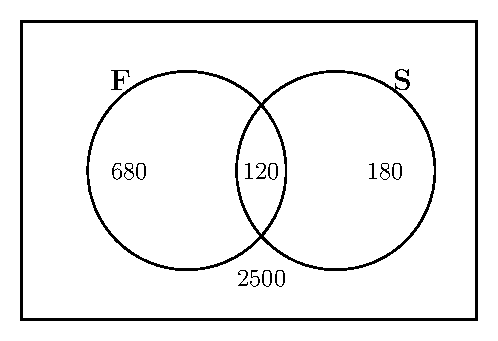
\includegraphics[width=0.7\textwidth]{figures/venn_conditional.pdf}
    \caption{Venn diagram showing football ($F$) and swimming ($S$) students at AUI.}
    \label{fig:venn_football_swim}
\end{figure}

\subsubsection*{Step a) Probability student plays football}
\[
P(F) = \frac{800}{3500} = \frac{8}{35}
\]

\subsubsection*{Step b) Probability student swims}
\[
P(S) = \frac{300}{3500} = \frac{3}{35}
\]

\subsubsection*{Step c) Probability student plays both football and swimming}
\[
P(F \cap S) = \frac{120}{3500} = \frac{6}{175}
\]

\subsubsection*{Step d) Probability student plays football or swims}
\[
P(F \cup S) = P(F) + P(S) - P(F \cap S) = \frac{7}{25}
\]

\subsubsection*{Step e) Probability student plays football given that they swim}
\[
P(F \mid S) = \frac{P(F \cap S)}{P(S)} = \frac{2}{5}
\]

\subsubsection*{Step f) Probability student plays football given that they do \textbf{not} swim}
\[
P(F \cap S^c) = P(F) - P(F \cap S) = \frac{34}{175}, \quad P(S^c) = 1 - P(S) = \frac{32}{35}
\]
\[
P(F \mid S^c) = \frac{P(F \cap S^c)}{P(S^c)} = \frac{17}{80}
\]

\subsubsection*{Step g) Probability student plays neither football nor swimming}
\[
P(F^c \cap S^c) = 1 - P(F \cup S) = \frac{18}{25}
\]

\subsubsection*{Step h) Probability student plays both football and swimming given they play at least one}
\[
P(F \cap S \mid F \cup S) = \frac{6}{49}
\]
\end{eg}

\begin{remark}
Conditional and joint probabilities, combined with independence checks, allow us to solve real-life problems such as sports participation by properly counting overlapping events.
\end{remark}

\section{Venn Diagram Probability Problems}

\subsection{Three-Set Venn Diagram}
\begin{definition}[Venn Diagram for Three Sets]
A Venn diagram represents three sets $A$, $B$, and $C$ and their relationships, including all possible intersections and complements. It is a visual tool to solve probability problems involving unions, intersections, and conditional probabilities.
\end{definition}

\begin{figure}[H]
    \centering
    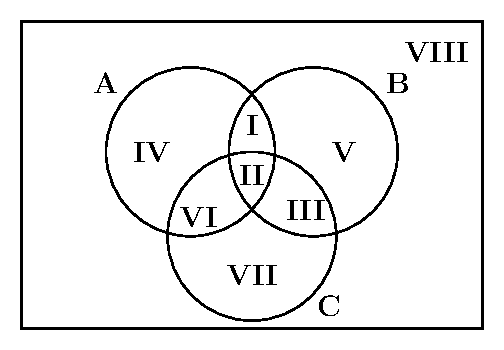
\includegraphics[width=0.6\textwidth]{figures/venn_3set.pdf}
    \caption{Three-set Venn diagram with labeled regions I--VIII.}
    \label{fig:venn3}
\end{figure}

\subsection{Region Labeling}
\begin{notation}
We assign Roman numerals I--VIII to each region in the Venn diagram as follows:
\begin{itemize}
    \item I: $A \cap B \cap C^c$ (A and B, not C)
    \item II: $A \cap B \cap C$ (all three sets)
    \item III: $A^c \cap B \cap C$ (B and C, not A)
    \item IV: $A \cap B^c \cap C^c$ (only A)
    \item V: $A^c \cap B \cap C^c$ (only B)
    \item VI: $A \cap B^c \cap C$ (A and C, not B)
    \item VII: $A^c \cap B^c \cap C$ (only C)
    \item VIII: $A^c \cap B^c \cap C^c$ (outside all sets)
\end{itemize}
\end{notation}

\subsection{Probability Solutions}
\begin{eg}[Venn Diagram Probabilities]
Let us solve the following probability problems using the labeled regions.

\paragraph{(a) Probability of $A$}
\[
P(A) = \text{I + II + IV + VI}
\]
\begin{explanation}
We sum all regions that include $A$.
\end{explanation}

\paragraph{(b) Probability of $A \cap C$}
\[
P(A \cap C) = \text{II + VI}
\]
\begin{explanation}
Only the regions that belong to both $A$ and $C$ are counted.
\end{explanation}

\paragraph{(c) Probability of $A \cup C$}
\[
P(A \cup C) = \text{I + II + III + IV + VI + VII}
\]

\paragraph{(d) Conditional Probability $P(A \mid B)$}
\[
P(A \mid B) = \frac{P(A \cap B)}{P(B)} = \frac{\text{I + II}}{\text{I + II + III + V}}
\]

\paragraph{(e) Conditional Probability $P(A \mid \overline{B \cap C})$}
\[
P(A \mid \overline{B \cap C}) = \frac{P(A \cap \overline{B \cap C})}{P(\overline{B \cap C})} = \frac{\text{I + IV + VI}}{\text{I + IV + V + VI + VII + VIII}}
\]

\paragraph{(f) Probability exactly one of $A$, $B$, or $C$ occurs}
\[
P(\text{exactly 1 of A, B, C}) = \text{IV + V + VII}
\]

\paragraph{(g) Conditional Probability $P(A \mid \overline{B} \cap C)$}
\[
P(A \mid \overline{B} \cap C) = \frac{P(A \cap \overline{B} \cap C)}{P(\overline{B} \cap C)} = \frac{\text{VI}}{\text{VI + VII}}
\]

\paragraph{(h) Conditional Probability of only $A$ given $A \cup B$}
\[
P(\text{only A} \mid A \cup B) = \frac{P(\text{only A})}{P(A \cup B)} = \frac{\text{IV}}{\text{I + II + III + IV + V + VI}}
\]

\begin{intuition}[Venn Diagram Approach]
Labeling regions helps systematically account for overlapping areas. By referring to regions with Roman numerals, we avoid double-counting and make conditional probabilities clear.
\end{intuition}

\end{eg}

\section{Important Probability Theorems}

\subsection{Total Probability Theorem}

\begin{theorem}[Total Probability Theorem]
Let $\{B_1, B_2, \ldots, B_n\}$ form a partition of the sample space $S$ (i.e., mutually exclusive and exhaustive). Then for any event $A$:
\[
P(A) = \sum_{i=1}^{n} P(A \mid B_i) \cdot P(B_i)
\]
\end{theorem}

\begin{proof}
Since $\{B_1, B_2, \ldots, B_n\}$ is a partition of $S$, we have
\[
A = A \cap S = A \cap \bigcup_{i=1}^{n} B_i = \bigcup_{i=1}^{n} (A \cap B_i)
\]
where the sets $A \cap B_i$ are mutually exclusive. By the \textbf{additivity of probability}:
\[
P(A) = \sum_{i=1}^{n} P(A \cap B_i)
\]
Using the definition of conditional probability, $P(A \cap B_i) = P(A \mid B_i) \cdot P(B_i)$. Substituting gives:
\[
P(A) = \sum_{i=1}^{n} P(A \mid B_i) \cdot P(B_i)
\]
\end{proof}

\begin{explanation}
The theorem allows us to compute the probability of $A$ by considering all “paths” $B_i$ through which $A$ can occur, then summing their contributions.
\end{explanation}

\begin{eg}[Special Case: Two Events]
For $B$ and its complement $B^c$:
\[
P(A) = P(A \mid B) \cdot P(B) + P(A \mid B^c) \cdot P(B^c)
\]
\end{eg}

\begin{eg}[Venn Diagram Example]
Using labeled Venn diagram regions:
\[
P(A) = \frac{\text{I + II}}{\text{I + II + III + V}} \cdot P(B) + \frac{\text{IV + VI}}{\text{IV + VI + VII + VIII}} \cdot P(B^c)
\]
\end{eg}

\begin{intuition}[Understanding Total Probability]
Think of the partition as splitting the sample space into mutually exclusive “paths” through which event $A$ can occur. Summing the contributions gives the total probability of $A$.
\end{intuition}

\subsection{Bayes' Theorem}

\begin{theorem}[Bayes' Theorem]
For any events $A$ and $B$ with $P(A) > 0$:
\[
P(B \mid A) = \frac{P(A \mid B) \cdot P(B)}{P(A)}
\]
\end{theorem}

\begin{proof}
By the definition of conditional probability:
\[
P(B \mid A) = \frac{P(B \cap A)}{P(A)} = \frac{P(A \cap B)}{P(A)}
\]
Using the definition of conditional probability again, $P(A \cap B) = P(A \mid B) \cdot P(B)$. Substituting gives:
\[
P(B \mid A) = \frac{P(A \mid B) \cdot P(B)}{P(A)}
\]
\end{proof}

\begin{explanation}
Bayes’ Theorem updates our belief about $B$ after observing $A$. It “flips” conditional probabilities, weighting by the prior probability of $B$.
\end{explanation}

\begin{eg}[Using Total Probability in Bayes]
If $\{B, B^c\}$ is a partition:
\[
P(B \mid A) = \frac{P(A \mid B) \cdot P(B)}{P(A \mid B) \cdot P(B) + P(A \mid B^c) \cdot P(B^c)}
\]
\end{eg}

\begin{eg}[General Partition]
For a partition $\{B_1, \ldots, B_n\}$:
\[
P(B_i \mid A) = \frac{P(A \mid B_i) \cdot P(B_i)}{\sum_{j=1}^{n} P(A \mid B_j) \cdot P(B_j)}
\]
\end{eg}

\begin{eg}[Venn Diagram Interpretation]
Using Venn diagram regions:
\[
P(B \mid A) = \frac{P(A \cap B)}{P(A)} = \frac{\text{I + II}}{\text{I + II + IV + VI}}
\]
\end{eg}

\begin{intuition}[Bayes Intuition]
Bayes’ Theorem allows us to answer: “Given we observed $A$, what is the probability that $B$ occurred?” It converts prior knowledge and likelihoods into updated beliefs.
\end{intuition}

\chapter{Counting}

\section{Combinatorics}

Probability problems often reduce to counting problems. By systematically enumerating outcomes, we can compute probabilities rigorously.

\subsection{Counting Principles}

\subsubsection{Multiplication Principle} 

\begin{explanation}
If a process consists of successive tasks, each of which can be performed in multiple ways, the total number of possible outcomes is the product of the number of ways to perform each task. This is sometimes called the \emph{Fundamental Counting Principle}.
\\
If task 1 can be done in $m_1$ ways, task 2 in $m_2$ ways, and task 3 in $m_3$ ways, then the total number of ways is $m_1 \cdot m_2 \cdot m_3$.
\end{explanation}


\begin{eg}[Dice Example]
Throw a four-sided die, then a six-sided die. Total outcomes:
\[
4 \times 6 = 24
\]

\begin{explanation}
We first choose the outcome of the first die (4 possibilities), then the second die (6 possibilities). Each choice of the first die can be paired with any of the second die outcomes, giving $4 \cdot 6 = 24$ total possibilities.
\end{explanation}
\end{eg}

\subsubsection{Addition Principle} 
\begin{explanation}
If a task can be completed by choosing one option from disjoint sets, the total number of ways is the sum of the number of ways in each set. This is essentially a "choose one among mutually exclusive options" principle.
\end{explanation}

\[
\text{If sets have } m_1, m_2, m_3 \text{ choices: } m_1 + m_2 + m_3
\]

\begin{eg}[Course Selection]
A student can choose a language course from either set A (3 courses) or set B (2 courses). Total choices:
\[
3 + 2 = 5
\]
\end{eg}

\subsubsection{Generalized Addition Principle (Inclusion–Exclusion)} 
\begin{explanation}
When sets are not disjoint, the \emph{Inclusion–Exclusion Principle} ensures we do not double-count overlapping elements.
\end{explanation}

\[
|A \cup B| = |A| + |B| - |A \cap B|
\]

\[
|A \cup B \cup C| = |A| + |B| + |C| - |A \cap B| - |A \cap C| - |B \cap C| + |A \cap B \cap C|
\]

\begin{proof}[Proof for Two Sets]
Each element in $A \cap B$ is counted twice when summing $|A| + |B|$. Subtracting $|A \cap B|$ corrects the overcount. This generalizes to three or more sets with alternating inclusion and exclusion.
\end{proof}

\begin{eg}[License Plates]
License plates can have format \texttt{nnllll} or \texttt{nlllll}, where $n$ is a digit ($0$–$9$) and $l$ is a lowercase letter ($a$–$z$).

\[
\text{\texttt{nnllll}}: 10^2 \cdot 26^4, \quad 
\text{\texttt{nlllll}}: 10 \cdot 26^5
\]

Total possibilities (disjoint formats):
\[
10^2 \cdot 26^4 + 10 \cdot 26^5
\]
\end{eg}

\subsubsection{Subtraction Principle (Complement Principle)}
\begin{explanation}
Sometimes it's easier to count what does \emph{not} happen and subtract from the total. This is often called the \emph{complement principle}.
\end{explanation}

\[
|S| = |U| - |\bar{S}|
\]

\begin{eg}[Strings Example]
Random string of length 6 from $\{a,b,c,d,e,f,g\}$. Probability it contains at least one of $\{a,b,c\}$?

\[
|U| = 7^6
\]

\[
|\bar{S}| = 4^6 \quad (\text{strings with no } a,b,c)
\]

\[
|S| = |U| - |\bar{S}| = 7^6 - 4^6
\]

\[
P(S) = \frac{|S|}{|U|} = \frac{7^6 - 4^6}{7^6}
\]

\begin{explanation}
Instead of counting all strings that contain $a$, $b$, or $c$ (complicated), we count strings without $a,b,c$ (simpler) and subtract from total.
\end{explanation}
\end{eg}

\subsubsection{Division Principle} 
\begin{explanation}
Used when objects are grouped into identical classes, or arrangements are indistinguishable in some way. If each object in $A$ corresponds to $k$ objects in $B$:

\[
|A| = \frac{|B|}{k}
\]
\end{explanation}

\begin{eg}[Seating Around a Table]
$5$ people around a circular table. Linear arrangements: $5! = 120$, but rotations are identical. Divide by $5$:
\[
\frac{5!}{5} = 24
\]
\end{eg}

\subsection{Common Discrete Structures}

\paragraph{1. Strings}  
Sequence of symbols. Number of strings of length $l$ from an alphabet of size $m$:
\[
m^l
\]

\paragraph{2. Permutations}
\begin{itemize}
    \item \textbf{All $n$ objects:} 
    \[
    n! = n \cdot (n-1) \cdot \dots \cdot 1
    \]

    \item \textbf{$k$ objects out of $n$:} 
    \[
    P(n,k) = \frac{n!}{(n-k)!} = n \cdot (n-1) \cdot \dots \cdot (n-k+1)
    \]

    \item \textbf{Example:} Arrange 3 objects from $\{a,b,c,d,e\}$:

    \[
    5 \cdot 4 \cdot 3 = 60 \text{ sequences}
    \]

    \begin{explanation}
    First pick the first object (5 options), then second (4 options), then third (3 options). Multiplication principle applies.
    \end{explanation}
\end{itemize}

\paragraph{3. Combinations / Selections}  
\begin{explanation}
Number of ways to select $k$ elements from $n$ distinct objects where order does not matter:
\[
\binom{n}{k} = \frac{n!}{k!(n-k)!}
\]
\end{explanation}

\begin{eg}[Selecting Students]
Choose 3 from $\{a,b,c,d,e\}$:
\[
\binom{5}{3} = 10
\]

\begin{explanation}
Order does not matter; $\{a,b,c\} = \{c,b,a\}$, so divide permutations $3!$ to remove overcounting.
\end{explanation}
\end{eg}

\paragraph{4. Permutations with Repetition}  
\begin{explanation}
When objects repeat, divide by factorials of repeated counts to avoid counting indistinguishable arrangements multiple times.
\end{explanation}

\begin{eg}[Name \texttt{Hamza}]
Letters: H,A,M,Z,A (two A's):
\[
\frac{5!}{2!} = 60
\]
\end{eg}
\begin{explanation}[General Formula]
$n$ objects with $n_1, n_2, \dots, n_k$ repetitions:
\[
\frac{n!}{n_1! \cdot n_2! \cdot \dots \cdot n_k!}
\]
\end{explanation}

\paragraph{5. Combinations with Repetition}  
\begin{explanation}
Selecting $k$ elements from $n$ types, allowing repetition:
\[
\binom{n+k-1}{k} = \frac{(n+k-1)!}{k!(n-1)!}
\]
\end{explanation}

\begin{eg}[Fruits Example]
Buy 4 fruits from 3 types (apples, oranges, bananas):
\[
\binom{3+4-1}{4} = \binom{6}{4} = 15
\]

Some possibilities: \{4 apples, 0 oranges, 0 bananas\}, \{3 apples, 1 orange, 0 bananas\}, \{2 apples, 2 oranges, 0 bananas\}, etc.
\end{eg}

\begin{proof}[Recursive Proof Using the "Stars and Bars" Idea]
Let $C(n,k)$ denote the number of ways to select $k$ elements from $n$ types with repetition.  

\textbf{Recursive idea:} Consider the first type of element (say apples). We can choose $0, 1, 2, \dots, k$ of them.  

- If we choose $i$ of the first type, we have $k-i$ elements left to choose from the remaining $n-1$ types.  
- By recursion, the number of ways for this case is $C(n-1, k-i)$.  

Hence, the recursion is:
\[
C(n,k) = \sum_{i=0}^{k} C(n-1, k-i)
\]

\textbf{Base cases:}  
\[
C(1,k) = 1 \quad \text{(all elements must be the only type)}, \qquad C(n,0) = 1 \quad \text{(choose nothing)}
\]

\textbf{Closed form via induction:} Assume the formula holds for $n-1$ types. Then:

\[
C(n,k) = \sum_{i=0}^{k} \binom{(n-1)+(k-i)-1}{k-i} = \sum_{i=0}^{k} \binom{n+k-i-3}{k-i}
\]

Using the standard identity
\[
\sum_{i=0}^{k} \binom{m+i}{i} = \binom{m+k+1}{k},
\]

we get
\[
C(n,k) = \binom{n+k-1}{k}.
\]

\end{proof}
\begin{remark}
Intuitively, each selection of $k$ items from $n$ types can be represented as $k$ stars and $n-1$ bars separating the types. Counting sequences of $k$ stars and $n-1$ bars gives exactly $\binom{n+k-1}{k}$.
\end{remark}

\begin{remark}[Counting Matrix for Sampling]
Here is a compact overview of the four classic counting cases in combinatorics:

\begin{table}[H]
\centering
\renewcommand{\arraystretch}{1.3} % increase row height
\setlength{\tabcolsep}{12pt} % increase column spacing
\begin{tabular}{lcc}
\toprule
 & \textbf{Without Repetition} & \textbf{With Repetition} \\
\midrule
\textbf{Ordered} & $P(n, r) = \dfrac{n!}{(n-r)!}$ & $n^r$ \\
\textbf{Unordered} & $\binom{n}{r} = \dfrac{n!}{r!(n-r)!}$ & $\binom{n+r-1}{r}$ \\
\bottomrule
\end{tabular}
\end{table}

\end{remark}

\begin{exercise}[Permutation Probability]
    For a random permutation of $\{1,2,3,4,5\}$, what is the probability that the first two digits sum to 5?

    The starting pairs summing to 5 are $(1,4), (4,1), (2,3),$ and $(3,2)$. There are 4 such pairs. The remaining 3 digits can be arranged in $3!$ ways.
    $$ P(\text{sum is 5}) = \frac{4 \times 3!}{5!} = \frac{24}{120} = \frac{1}{5} $$
\end{exercise}

\begin{exercise}[Committee Selection]
    A committee of 6 is chosen from 20 Moroccan and 10 foreign professors. Find the probability of selecting: a) exactly 2 foreign professors, and b) at least 2 foreign professors.

    a) For exactly 2 foreign (and 4 Moroccan) professors:
    $$ P(\text{exactly 2 foreign}) = \frac{\binom{10}{2}\binom{20}{4}}{\binom{30}{6}} \approx 0.3672 $$
    b) For at least 2 foreign professors, we use the complement rule:
    $$ P(\ge 2) = 1 - P(0 \text{ or } 1 \text{ foreign}) = 1 - \frac{\binom{10}{0}\binom{20}{6} + \binom{10}{1}\binom{20}{5}}{\binom{30}{6}} \approx 0.6736 $$
\end{exercise}

\begin{exercise}[Weighted String Probability]
    A 4-digit string is made from $\{1,2,3\}$. The probability of a string $x$ is proportional to its first digit $x_1$. Find the probability that the string is: a) all the same digit, and b) a palindrome.

    The probability of any string $x$ is $P(x) = x_1/162$.
    
    a) All digits are the same ('1111', '2222', '3333'):
    $$ P(\text{all same}) = \frac{1}{162} + \frac{2}{162} + \frac{3}{162} = \frac{6}{162} = \frac{1}{27} $$
    b) The string is a palindrome (form $x_1x_2x_2x_1$):
    $$ P(\text{palindrome}) = \frac{3 \times 1 + 3 \times 2 + 3 \times 3}{162} = \frac{3(1+2+3)}{162} = \frac{18}{162} = \frac{1}{9} $$
\end{exercise}

\begin{exercise}
    Consider picking a permutation of 12233 with equal likelihood
    \[
    P(\text{perm has 2 symbols adding up to 4})
    \]
\end{exercise}

\begin{exercise}
    Consider all solutions to 
    \[
    x_1 + x_2 + x_3 + x_4 = 10
    \]
    Pick any one of them with equal likelihood
    \begin{enumerate}
        \item $P(\text{exactly 3 of the $x_i$'have the same value}) = $
        \item $P(\text{all 4 of them have the same value}) =$
        \item $P(x_1 = 3) = $
    \end{enumerate}
\end{exercise}




\chapter{Random Variables}
\addtolength{\topmargin}{-0.9pt}

\section{Basic Concepts}

\begin{definition}[Random Variable]
A \emph{random variable} is a function 
\[
X : \samplespace \to \mathbb{R}
\]
from the sample space \( \samplespace \) of an experiment to the set of real numbers \( \mathbb{R} \).
\end{definition}

\begin{eg}
Suppose we choose \(3\) elements from the set \(\{1,2,\dots,6\}\) uniformly at random.  
Then the sample space is 
\[
\samplespace = \{ \{1,2,3\}, \{1,2,4\}, \dots, \{4,5,6\} \},
\]
and 
\[
|\samplespace| = \binom{6}{3} = 20.
\]

\begin{enumerate}[label=(\alph*)]
    \item Define a random variable 
    \[
    X : \samplespace \to \mathbb{R}, \quad X(\{a,b,c\}) = \max(a,b,c).
    \]
    Then 
    \[
    \text{Range}(X) = \{3,4,5,6\}.
    \]
    
    \item Define another random variable 
    \[
    Y : \samplespace \to \mathbb{R}, \quad Y(\{a,b,c\}) = \frac{a+b+c}{3}.
    \]
    Then 
    \[
    \text{Range}(Y) = \{2, 2.5, 3, 3.5, 4, 4.5, 5\}.
    \]
\end{enumerate}
\end{eg}

\begin{eg}
Consider all permutations of the numbers \(1,2,3,4,5\).  
Define the random variable
\[
Z(\pi) = \#\{ i \in \{1,\dots,5\} : \pi(i) \neq i \},
\]
the number of elements that are \emph{not} in their original position (i.e., the number of displaced elements).

For example:
\[
Z(12345) = 0, \qquad Z(12453) = 2.
\]
\end{eg}

\begin{eg}
You have \(5\) cameras, of which \(2\) work and \(3\) do not.  
You mix them up and test them one by one until you find a working one.  
Let the random variable \(W\) be the number of cameras tested.

Then the range of \(W\) is
\[
\text{Range}(W) = \{1,2,3\},
\]
since the first working camera could appear in the first, second, or third test at most (after testing 3 failed ones, you are guaranteed a working one next).
\end{eg}

\begin{definition}[Probability Mass Function]
Let \(X\) be a discrete random variable with range
\[
R_X = \{x_1, x_2, x_3, \ldots\},
\]
where \(R_X\) is finite or countably infinite.  
The \emph{probability mass function (PMF)} of \(X\) is the function
\[
p_X(x) = \Pr(X = x), \quad x \in \mathbb{R}.
\]
The PMF satisfies:
\[
p_X(x) \ge 0 \quad \forall x, 
\qquad \sum_{x \in R_X} p_X(x) = 1.
\]
\end{definition}

\begin{eg}
Continuing from Example 1, let \( X = \max(a,b,c) \).  
To find its PMF, note that:

\begin{itemize}
    \item For \(X = 3\): the only possible subset is \(\{1,2,3\}\), so \(\Pr(X=3) = \frac{1}{20}\).
    \item For \(X = 4\): we must have \(4\) included and the other two from \(\{1,2,3\}\), giving \(\binom{3}{2} = 3\) subsets, so \(\Pr(X=4) = \frac{3}{20}\).
    \item For \(X = 5\): we must have \(5\) included and the other two from \(\{1,2,3,4\}\), giving \(\binom{4}{2} = 6\) subsets, so \(\Pr(X=5) = \frac{6}{20}\).
    \item For \(X = 6\): we must have \(6\) included and the other two from \(\{1,2,3,4,5\}\), giving \(\binom{5}{2} = 10\) subsets, so \(\Pr(X=6) = \frac{10}{20} = \frac{1}{2}\).
\end{itemize}

Hence,
\[
f_X(x) =
\begin{cases}
\dfrac{1}{20}, & x = 3, \\[6pt]
\dfrac{3}{20}, & x = 4, \\[6pt]
\dfrac{6}{20}, & x = 5, \\[6pt]
\dfrac{10}{20}, & x = 6, \\[6pt]
0, & \text{otherwise.}
\end{cases}
\]

We can verify normalization:
\[
\frac{1 + 3 + 6 + 10}{20} = \frac{20}{20} = 1.
\]
\end{eg}

\begin{eg}
You have \(5\) cameras, of which \(2\) work and \(3\) do not.  
You mix them up and test them one by one until you find a working one.  
Let the random variable \(W\) be the number of cameras tested.

Then the range of \(W\) is
\[
\text{Range}(W) = \{1,2,3\},
\]
since the first working camera could appear in the first, second, or third test at most (after testing \(3\) failed ones, you are guaranteed a working one next).

We can compute the probability mass function \(p_W(k) = P(W = k)\) as follows.

\[
f_W(w) =
\begin{cases}
\dfrac{2}{5}, & w = 1, \\[1em]
\dfrac{3}{5}\cdot\dfrac{2}{4} = \dfrac{3}{10}, & w = 2, \\[1em]
\dfrac{3}{5}\cdot\dfrac{2}{4} = \dfrac{6}{20}, & w = 3, \\[1em]
0, & \text{otherwise.}
\end{cases}
\]

\textbf{Verification:}
\[
\frac{2}{5} + \frac{3}{10} + \frac{6}{20} = 1,
\]
so the PMF is valid.
\end{eg}

\begin{eg}
    Throw a 4-sided die until you get a ``3''.  
    Let the random variable \( X \) be the number of throws required to get the first ``3''.  

    \[
    \text{Range}(X) = \mathbb{N} = \{1, 2, 3, \dots\}.
    \]

    The probability of success (getting a ``3'') on any single throw is \( p = \dfrac{1}{4} \),  
    and the probability of failure is \( q = 1 - p = \dfrac{3}{4} \).

    \begin{enumerate}[label=(\alph*)]
        \item For \( X = 8 \):
        \[
        f_X(8) = P(X = 8) = q^{8-1}p = \left(\dfrac{3}{4}\right)^{7} \left(\dfrac{1}{4}\right).
        \]

        \item In general, for the geometric distribution:
        \[
        f_X(k) = P(X = k) = q^{k-1}p = 
        \left( \dfrac{3}{4} \right)^{k-1} 
        \left( \dfrac{1}{4} \right),
        \quad k = 1, 2, 3, \dots
        \]

        \item To verify that \( f_X \) is a valid PMF:
        \[
        \sum_{k=1}^{\infty} f_X(k)
        = \sum_{k=1}^{\infty} \left( \dfrac{3}{4} \right)^{k-1} 
        \left( \dfrac{1}{4} \right)
        = \dfrac{1}{4} \sum_{k=0}^{\infty} 
        \left( \dfrac{3}{4} \right)^k
        = \dfrac{1}{4} \cdot \dfrac{1}{1 - \frac{3}{4}}
        = 1.
        \]
    \end{enumerate}
\end{eg}


\section{More on discrete random variables}

\begin{definition}[Cumulative Distribution Function]
    The \emph{cumulative distribution function (CDF)} of a random variable \( X \) is defined as
    \[
        F_X(x) = P(X \le x), \quad \forall x \in \mathbb{R}.
    \]
\end{definition}

\begin{eg}
    Let \(Y\) be a discrete random variable with probability mass function \(f_Y(y)\) given by

    \[
    f_Y(y) =
    \begin{cases}
        \dfrac{1}{15}, & y = -1, \\[3mm]
        \dfrac{3}{15}, & y = 0, \\[3mm]
        \dfrac{4}{15}, & y = 2, \\[3mm]
        \dfrac{2}{15}, & y = 6, \\[3mm]
        \dfrac{5}{15}, & y = 10, \\[3mm]
        0, & \text{otherwise}.
    \end{cases}
    \]

    \begin{enumerate}[label=(\alph*)]
        \item Verify that this is a valid PMF:  
        \[
        \frac{1}{15} + \frac{3}{15} + \frac{4}{15} + \frac{2}{15} + \frac{5}{15} = \frac{15}{15} = 1.
        \]

        \item Compute the CDF \(F_Y(y) = P(Y \le y)\):
        \[
        F_Y(y) =
        \begin{cases}
            0, & y < -1, \\[1mm]
            \frac{1}{15}, & -1 \le y < 0, \\[2mm]
            \frac{4}{15}, & 0 \le y < 2, \\[2mm]
            \frac{8}{15}, & 2 \le y < 6, \\[2mm]
            \frac{10}{15}, & 6 \le y < 10, \\[2mm]
            1, & y \ge 10.
        \end{cases}
        \]
    \end{enumerate}
\end{eg}


\begin{remark}
The probability mass function (PMF) and the cumulative distribution function (CDF) describe a random variable in related but distinct ways.

\begin{center}
\renewcommand{\arraystretch}{1.2}
\begin{tabular}{c|ccc}
\hline
\textbf{Aspect} & \textbf{PMF} & \textbf{CDF} \\ \hline
Symbol & $p_X(x)$ & $F_X(x)$ \\ \hline
Definition & $p_X(x)=P(X=x)$ & $F_X(x)=P(X\le x)$ \\ \hline
Domain & Discrete $x$ & Real $x$ \\ \hline
Range & $[0,1]$ & $[0,1]$ \\ \hline
Relation & $F_X(x)=\sum_{t\le x}p_X(t)$ & $p_X(x)=F_X(x)-F_X(x^-)$ \\ \hline
Nature & Stepwise (non-continuous) & Non-decreasing, right-continuous \\ \hline
\end{tabular}
\end{center}
\end{remark}


% exmaples, check phones for picture. 



\begin{exercise}
$X$ is uniform over $[0,5] \cup [10,20]$. Find $F_X(x)$ and draw it.
\end{exercise}

\begin{proof}
The total length of the support is $5 + 10 = 15$.

The cumulative distribution function is:
\[
F_X(x) = \begin{cases}
0 & x < 0 \\
\frac{x}{15} & 0 \leq x < 5 \\
\frac{5}{15} = \frac{1}{3} & 5 \leq x < 10 \\
\frac{5 + (x-10)}{15} = \frac{x-5}{15} & 10 \leq x < 20 \\
1 & x \geq 20
\end{cases}
\]

\begin{center}
\begin{tikzpicture}
\begin{axis}[
    axis lines = center,
    xlabel = {$x$},
    ylabel = {$F_X(x)$},
    xmin=-1, xmax=22,
    ymin=-0.1, ymax=1.2,
    xtick={0,5,10,20},
    ytick={0,0.333,1},
    yticklabels={0,$\frac{1}{3}$,1},
    width=10cm,
    height=6cm
]
\addplot[domain=-1:0, blue, thick] {0};
\addplot[domain=0:5, blue, thick] {x/15};
\addplot[domain=5:10, blue, thick] {1/3};
\addplot[domain=10:20, blue, thick] {(x-5)/15};
\addplot[domain=20:22, blue, thick] {1};
\end{axis}
\end{tikzpicture}
\end{center}
\end{proof}

\begin{exercise}
$Y$ has range $[0,10] \cup [20,25]$. It is uniform over $[0,10]$ and uniform over $[20,25]$ with $P(10 \leq Y \leq 25) = 3 \cdot P(0 \leq Y \leq 10)$. Find $F_Y$
$X$ is uniform over $[0,5] \cup [10,20]$. Find $f_X(x)$ and draw it.
\end{exercise}

\begin{proof}
The total length of the support is $(5 - 0) + (20 - 10) = 15$.
For a uniform distribution, the pdf $f_X(x)$ is $1/(\text{Total Length})$ over the support, and $0$ elsewhere.
\[
f_X(x) = \begin{cases}
\frac{1}{15} & 0 \leq x \leq 5 \\
\frac{1}{15} & 10 \leq x \leq 20 \\
0 & \text{otherwise}
\end{cases}
\]

\begin{center}
\begin{tikzpicture}
\begin{axis}[
    axis lines = center,
    xlabel = {$x$},
    ylabel = {$f_X(x)$},
    xmin=-1, xmax=22,
    ymin=-0.05, ymax=0.15,
    xtick={0,5,10,20},
    ytick={0.0667},
    yticklabels={$\frac{1}{15}$},
    width=10cm,
    height=5cm
]
\addplot[blue, thick, domain=-1:0] {0};
\addplot[blue, thick, domain=0:5] {1/15};
\addplot[blue, thick, domain=5:10] {0};
\addplot[blue, thick, domain=10:20] {1/15};
\addplot[blue, thick, domain=20:22] {0};
% Vertical lines to close the boxes
\draw[blue, thick] (axis cs:0,0) -- (axis cs:0,0.0667);
\draw[blue, thick] (axis cs:5,0.0667) -- (axis cs:5,0);
\draw[blue, thick] (axis cs:10,0) -- (axis cs:10,0.0667);
\draw[blue, thick] (axis cs:20,0.0667) -- (axis cs:20,0);
\end{axis}
\end{tikzpicture}
\end{center}
\end{proof}

\begin{exercise}
$Y$ has range $[0,10] \cup [20,25]$. It is uniform over $[0,10]$ and uniform over $[20,25]$ with $P(20 \leq Y \leq 25) = 3 \cdot P(0 \leq Y \leq 10)$. Find $F_Y(y)$.
\end{exercise}

\begin{proof}
Let $P(0 \leq Y \leq 10) = p_1$ and $P(20 \leq Y \leq 25) = p_2$.
Given: $p_1 + p_2 = 1$ and $p_2 = 3p_1$.
Substituting gives $p_1 + 3p_1 = 1 \implies 4p_1 = 1 \implies p_1 = \frac{1}{4}$ and $p_2 = \frac{3}{4}$.

We find the pdf $f_Y(y)$ heights.
For $0 \leq y \leq 10$ (length 10): $\int_0^{10} c_1 \, dy = p_1 \implies 10 c_1 = \frac{1}{4} \implies c_1 = \frac{1}{40}$.
For $20 \leq y \leq 25$ (length 5): $\int_{20}^{25} c_2 \, dy = p_2 \implies 5 c_2 = \frac{3}{4} \implies c_2 = \frac{3}{20}$.

Now, we find the CDF $F_Y(y) = \int_{-\infty}^y f_Y(t) \, dt$:
\[
F_Y(y) = \begin{cases}
0 & y < 0 \\
\int_0^y \frac{1}{40} \, dt = \frac{y}{40} & 0 \leq y < 10 \\
F_Y(10) = \frac{10}{40} = \frac{1}{4} & 10 \leq y < 20 \\
F_Y(20) + \int_{20}^y \frac{3}{20} \, dt = \frac{1}{4} + \frac{3(y-20)}{20} & 20 \leq y < 25 \\
F_Y(25) = \frac{1}{4} + \frac{3(25-20)}{20} = \frac{1}{4} + \frac{15}{20} = 1 & y \geq 25
\end{cases}
\]
\end{proof}

\begin{exercise}
Random variable $Z$ has range $[0,4]$ with $f_Z(z) = Cz^2$. Find $c$.
\begin{center}
\begin{tikzpicture}
\begin{axis}[
    axis lines = center,
    xlabel = {$z$},
    ylabel = {$f_Z(z)$},
    xmin=-0.5, xmax=4.5,
    ymin=-0.05, ymax=0.9,
    xtick={0,4},
    ytick={0.75},
    yticklabels={$\frac{3}{4}$},
    width=8cm,
    height=6cm,
    samples=100
]
\addplot[blue, thick, domain=0:4] {(3/64)*x^2};
\node[above left] at (axis cs:3, { (3/64)*3^2 }) {$f_Z(z) = Cz^2$};
\addplot[dashed, domain=0:4, opacity=0.5] coordinates {(4,0) (4, 0.75)};
\end{axis}
\end{tikzpicture}
\end{center}
\end{exercise}

\begin{proof}
For $f_Z(z)$ to be a valid pdf, its integral over its range $[0,4]$ must be 1.
\[
\int_0^4 Cz^2 \, dz = 1
\]
\[
C \left[ \frac{z^3}{3} \right]_0^4 = 1
\]
\[
C \left( \frac{4^3}{3} - \frac{0^3}{3} \right) = 1
\]
\[
C \left( \frac{64}{3} \right) = 1 \implies c = \frac{3}{64}
\]
(The peak value at $z=4$ is $f_Z(4) = \frac{3}{64}(4^2) = \frac{3 \cdot 16}{64} = \frac{48}{64} = \frac{3}{4}$.)
\end{proof}

\begin{exercise}
Random variable $W$ has the following pdf. Find $f_W(w)$.
\begin{center}
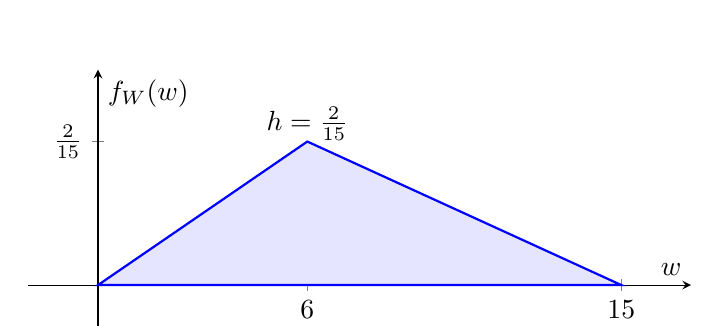
\begin{tikzpicture}
\begin{axis}[
    axis lines = center,
    xlabel = {$w$},
    ylabel = {$f_W(w)$},
    xmin=-2, xmax=17,
    ymin=-0.05, ymax=0.2,
    xtick={0,6,15},
    ytick={0.1333},
    yticklabels={$\frac{2}{15}$},
    width=10cm,
    height=5cm
]
\addplot[blue, thick, fill=blue!10] coordinates {(0,0) (6, 0.1333) (15,0) (0,0)} -- cycle;
\node at (axis cs:6, 0.15) {$h = \frac{2}{15}$};
\end{axis}
\end{tikzpicture}
\end{center}
\end{exercise}

\begin{proof}
The pdf is a triangle with base $b=15$. The area must be 1, so $\frac{1}{2} \cdot 15 \cdot h = 1$, which gives the height $h = \frac{2}{15}$ at the peak $w=6$.

We find the equations for the two lines:
\begin{itemize}
    \item \textbf{Line 1 ($0 \leq w < 6$):} Passes through $(0,0)$ and $(6, 2/15)$.
    Slope $m_1 = \frac{2/15}{6} = \frac{1}{45}$.
    Equation: $f_W(w) = \frac{1}{45}w$.
    
    \item \textbf{Line 2 ($6 \leq w \leq 15$):} Passes through $(6, 2/15)$ and $(15, 0)$.
    Slope $m_2 = \frac{0 - 2/15}{15 - 6} = -\frac{2}{135}$.
    Using point $(15,0)$: $f_W(w) = -\frac{2}{135}(w - 15) = \frac{2}{9} - \frac{2}{135}w$.
\end{itemize}

\[
f_W(w) = \begin{cases}
\frac{1}{45}w & 0 \leq w < 6 \\
\frac{2}{9} - \frac{2}{135}w & 6 \leq w \leq 15 \\
0 & \text{otherwise}
\end{cases}
\]
\end{proof}



\begin{exercise}
\begin{center}
\begin{tikzpicture}[scale=0.6]
    % Axes
    \draw[->] (0,0) -- (17,0) node[right] {$x$};
    \draw[->] (0,0) -- (0,5) node[above] {$f_X(x)$};
    
    % Piecewise PDF
    \draw[thick] (0,0) -- (6,3); % sloped part
    \draw[thick] (6,3) -- (15,3); % flat part

    % Labels
    \node[below] at (6,0) {6};
    \node[below] at (15,0) {15};
\end{tikzpicture}
\end{center}

\begin{enumerate}[label=(\alph*)]
    \item Write down \( f_X(x) \).

    \item Calculate the following probabilities:
    \begin{enumerate}[label=(\roman*)]
        \item \( P(X \le 6) \)
        \item \( P(X \ge 6) \)
        \item \( P(4 \le X \le 12) \)
        \item \( P(|X - 6| \le 2) \)
    \end{enumerate}
\end{enumerate}
\end{exercise}

\begin{exercise}
Consider the density sketched below: it is linear from \(x=0\) to \(x=6\) reaching height \(h\) at \(x=6\), constant equal to \(h\) on \([6,15]\), and zero elsewhere.

\begin{center}
% (simple schematic)
\begin{tikzpicture}[scale=0.6]
  \draw[->] (0,0) -- (16,0) node[right] {$x$};
  \draw[->] (0,0) -- (0,3.6) node[above] {$f_X(x)$};
  \draw[thick] (0,0) -- (6,2) -- (15,2) -- (15,0);
  \node[below] at (6,0) {6};
  \node[below] at (15,0) {15};
  \node[left] at (0,2) {$h$};
\end{tikzpicture}
\end{center}

\begin{enumerate}[label=(\alph*)]
  \item Write down \(f_X(x)\).
  \item Calculate the following probabilities:
  \begin{enumerate}[label=(\roman*)]
    \item \(P(X\le 6)\)
    \item \(P(X\ge 6)\)
    \item \(P(4\le X\le 12)\)
    \item \(P(|X-6|\le 2)\)
  \end{enumerate}
\end{enumerate}
\end{exercise}

\begin{solution}
1. find \(h\) and the piecewise form of \(f_X\).
The total area must equal \(1\). The area is the triangle on \([0,6]\) plus the rectangle on \([6,15]\):
\[
\frac{1}{2}\cdot 6\cdot h \;+\; 9\cdot h \;=\; 3h + 9h = 12h = 1
\quad\Longrightarrow\quad h=\frac{1}{12}.
\]
On \([0,6]\) the density is linear from \(0\) to \(h\). Its slope is \(h/6\), so for \(0\le x\le6\)
\[
f_X(x)=\frac{h}{6}\,x=\frac{1}{12}\cdot\frac{x}{6}=\frac{x}{72}.
\]
On \([6,15]\), \(f_X(x)=h=\tfrac{1}{12}\). Elsewhere \(f_X(x)=0\). Thus
\[
f_X(x)=
\begin{cases}
\dfrac{x}{72}, & 0\le x\le 6,\\[6pt]
\dfrac{1}{12}, & 6<x\le 15,\\[4pt]
0, & \text{otherwise.}
\end{cases}
\]

2. probabilities.
(i) \(P(X\le6)\) is the area of the triangle:
\[
P(X\le6)=\tfrac{1}{2}\cdot 6\cdot h=3h=3\cdot\frac{1}{12}=\frac{1}{4}.
\]

(ii) \(P(X\ge6)\) is the area of the rectangle \([6,15]\):
\[
P(X\ge6)=9\cdot h=9\cdot\frac{1}{12}=\frac{3}{4}.
\]
(For a continuous distribution the inclusion of the endpoint does not matter.)

(iii) \(P(4\le X\le12)\). Split at \(6\):
\[
P(4\le X\le12)=\int_{4}^{6}\frac{x}{72}\,dx+\int_{6}^{12}\frac{1}{12}\,dx.
\]
Compute each term:
\[
\int_{4}^{6}\frac{x}{72}\,dx=\left.\frac{x^2}{144}\right|_{4}^{6}=\frac{36-16}{144}=\frac{20}{144}=\frac{5}{36},
\]
\[
\int_{6}^{12}\frac{1}{12}\,dx=\frac{1}{12}\cdot(12-6)=\frac{6}{12}=\frac{1}{2}.
\]
So
\[
P(4\le X\le12)=\frac{5}{36}+\frac{1}{2}=\frac{5+18}{36}=\frac{23}{36}.
\]
(iv) \(P(|X-6|\le2)=P(4\le X\le8)\). Split at \(6\):
\[
P(4\le X\le8)=\int_{4}^{6}\frac{x}{72}\,dx+\int_{6}^{8}\frac{1}{12}\,dx.
\]
We already have \(\int_{4}^{6}\frac{x}{72}\,dx=\frac{5}{36}\). The second integral is
\[
\int_{6}^{8}\frac{1}{12}\,dx=\frac{1}{12}\cdot(8-6)=\frac{2}{12}=\frac{1}{6}=\frac{6}{36}.
\]
Thus
\[
P(|X-6|\le2)=\frac{5}{36}+\frac{6}{36}=\frac{11}{36}.
\]
\end{solution}


% bell curves, expectation, probability course .com distribution rand varss
\chapter{Discrete Joint Distributions}
\addtolength{\topmargin}{-0.9pt}

\section{Basic Concepts}
\index{joint distribution}
\index{joint PMF}

\begin{definition}[Joint Probability Mass Function]\index{joint PMF|see{joint probability mass function}}
Let $X$ and $Y$ be discrete random variables. The \emph{joint probability mass function (joint PMF)} of $X$ and $Y$ is defined as:
\[
p_{X,Y}(x, y) = P(X = x \text{ and } Y = y), \quad \text{for all } x, y
\]

The joint PMF satisfies:
\begin{enumerate}
    \item $p_{X,Y}(x, y) \geq 0$ for all $x, y$
    \item $\sum_{x} \sum_{y} p_{X,Y}(x, y) = 1$
\end{enumerate}
\end{definition}

\begin{definition}[Marginal PMF]\index{marginal PMF}
The \emph{marginal PMF} of $X$ is:
\[
p_X(x) = \sum_{y} p_{X,Y}(x, y)
\]

Similarly, the marginal PMF of $Y$ is:
\[
p_Y(y) = \sum_{x} p_{X,Y}(x, y)
\]
\end{definition}

\begin{exercise}[DIY: Marginals Sum to 1]
Prove that if $p_{X,Y}(x, y)$ is a valid joint PMF, then:
\[
\sum_{x} p_X(x) = 1 \quad \text{and} \quad \sum_{y} p_Y(y) = 1
\]
\end{exercise}

\begin{proof}
\[
\sum_{x} p_X(x) = \sum_{x} \sum_{y} p_{X,Y}(x, y) = 1
\]
since the joint PMF sums to 1. Similarly:
\[
\sum_{y} p_Y(y) = \sum_{y} \sum_{x} p_{X,Y}(x, y) = 1
\]
\end{proof}

\begin{eg}[Simple Joint Distribution]
Consider two random variables $X$ and $Y$ with the following joint PMF:

\begin{center}
\renewcommand{\arraystretch}{1.5}
\begin{tabular}{c|ccc}
$p_{X,Y}(x,y)$ & $X=1$ & $X=2$ & $X=3$ \\ \hline
$Y=2$ & 0.1 & 0.2 & 0.1 \\
$Y=3$ & 0.15 & 0.15 & 0.1 \\
$Y=4$ & 0.05 & 0.1 & 0.05 \\
\end{tabular}
\end{center}

Find:
\begin{enumerate}[label=(\alph*)]
    \item The marginal PMFs of $X$ and $Y$
    \item $P(X = 2)$
    \item $P(Y \geq 3)$
    \item $P(X = 2, Y = 3)$
\end{enumerate}

\begin{solution}
\begin{enumerate}[label=(\alph*)]
    \item \textbf{Marginal PMF of $X$:}
    \[
    p_X(1) = 0.1 + 0.15 + 0.05 = 0.3, \quad p_X(2) = 0.2 + 0.15 + 0.1 = 0.45, \quad p_X(3) = 0.1 + 0.1 + 0.05 = 0.25
    \]
    
    \textbf{Marginal PMF of $Y$:}
    \[
    p_Y(2) = 0.1 + 0.2 + 0.1 = 0.4, \quad p_Y(3) = 0.15 + 0.15 + 0.1 = 0.4, \quad p_Y(4) = 0.05 + 0.1 + 0.05 = 0.2
    \]
    
    \item $P(X = 2) = p_X(2) = 0.45$
    
    \item $P(Y \geq 3) = p_Y(3) + p_Y(4) = 0.4 + 0.2 = 0.6$
    
    \item $P(X = 2, Y = 3) = p_{X,Y}(2, 3) = 0.15$
\end{enumerate}
\end{solution}
\end{eg}

\section{Conditional Distributions}
\index{conditional distribution}
\index{conditional PMF}

\begin{definition}[Conditional PMF]
The \emph{conditional PMF} of $Y$ given $X = x$ is:
\[
p_{Y|X}(y \mid x) = \frac{p_{X,Y}(x, y)}{p_X(x)}, \quad \text{provided } p_X(x) > 0
\]

Similarly, the conditional PMF of $X$ given $Y = y$ is:
\[
p_{X|Y}(x \mid y) = \frac{p_{X,Y}(x, y)}{p_Y(y)}, \quad \text{provided } p_Y(y) > 0
\]
\end{definition}

\begin{exercise}[DIY: Conditional PMF is Valid PMF]
Prove that for a fixed $x$ with $p_X(x) > 0$, the conditional PMF $p_{Y|X}(y \mid x)$ satisfies:
\begin{enumerate}[label=(\alph*)]
    \item $p_{Y|X}(y \mid x) \geq 0$ for all $y$
    \item $\sum_{y} p_{Y|X}(y \mid x) = 1$
\end{enumerate}
\end{exercise}

\begin{proof}
\begin{enumerate}[label=(\alph*)]
    \item Since $p_{X,Y}(x, y) \geq 0$ and $p_X(x) > 0$, we have $p_{Y|X}(y \mid x) = \frac{p_{X,Y}(x, y)}{p_X(x)} \geq 0$.
    
    \item 
    \[
    \sum_{y} p_{Y|X}(y \mid x) = \sum_{y} \frac{p_{X,Y}(x, y)}{p_X(x)} = \frac{1}{p_X(x)} \sum_{y} p_{X,Y}(x, y) = \frac{p_X(x)}{p_X(x)} = 1
    \]
\end{enumerate}
\end{proof}

\begin{eg}[Conditional Distributions]
Using the joint distribution from the previous example, find:
\begin{enumerate}[label=(\alph*)]
    \item $p_{Y|X}(y \mid 2)$ (the conditional PMF of $Y$ given $X = 2$)
    \item $p_{X|Y}(x \mid 3)$ (the conditional PMF of $X$ given $Y = 3$)
    \item $P(Y = 4 \mid X = 1)$
\end{enumerate}

\begin{solution}
\begin{enumerate}[label=(\alph*)]
    \item Given $X = 2$, we have $p_X(2) = 0.45$:
    \[
    p_{Y|X}(2 \mid 2) = \frac{0.2}{0.45} = \frac{4}{9}, \quad p_{Y|X}(3 \mid 2) = \frac{0.15}{0.45} = \frac{1}{3}, \quad p_{Y|X}(4 \mid 2) = \frac{0.1}{0.45} = \frac{2}{9}
    \]
    
    \item Given $Y = 3$, we have $p_Y(3) = 0.4$:
    \[
    p_{X|Y}(1 \mid 3) = \frac{0.15}{0.4} = \frac{3}{8}, \quad p_{X|Y}(2 \mid 3) = \frac{0.15}{0.4} = \frac{3}{8}, \quad p_{X|Y}(3 \mid 3) = \frac{0.1}{0.4} = \frac{1}{4}
    \]
    
    \item $P(Y = 4 \mid X = 1) = p_{Y|X}(4 \mid 1) = \frac{p_{X,Y}(1, 4)}{p_X(1)} = \frac{0.05}{0.3} = \frac{1}{6}$
\end{enumerate}
\end{solution}
\end{eg}

\section{Independence}
\index{independence!discrete random variables}

\begin{definition}[Independence]
Two discrete random variables $X$ and $Y$ are \emph{independent} if and only if:
\[
p_{X,Y}(x, y) = p_X(x) \cdot p_Y(y) \quad \text{for all } x, y
\]

Equivalently, $X$ and $Y$ are independent if:
\[
p_{Y|X}(y \mid x) = p_Y(y) \quad \text{for all } x, y \text{ with } p_X(x) > 0
\]
\end{definition}

\begin{exercise}[DIY: Equivalence of Independence Definitions]
Prove that the two definitions of independence are equivalent:
\begin{enumerate}[label=(\alph*)]
    \item If $p_{X,Y}(x, y) = p_X(x) \cdot p_Y(y)$ for all $x, y$, then $p_{Y|X}(y \mid x) = p_Y(y)$ for all $x, y$ with $p_X(x) > 0$.
    \item If $p_{Y|X}(y \mid x) = p_Y(y)$ for all $x, y$ with $p_X(x) > 0$, then $p_{X,Y}(x, y) = p_X(x) \cdot p_Y(y)$ for all $x, y$.
\end{enumerate}
\end{exercise}

\begin{proof}
\begin{enumerate}[label=(\alph*)]
    \item If $p_{X,Y}(x, y) = p_X(x) \cdot p_Y(y)$, then:
    \[
    p_{Y|X}(y \mid x) = \frac{p_{X,Y}(x, y)}{p_X(x)} = \frac{p_X(x) \cdot p_Y(y)}{p_X(x)} = p_Y(y)
    \]
    provided $p_X(x) > 0$.
    
    \item If $p_{Y|X}(y \mid x) = p_Y(y)$ for all $x, y$ with $p_X(x) > 0$, then:
    \[
    p_{X,Y}(x, y) = p_{Y|X}(y \mid x) \cdot p_X(x) = p_Y(y) \cdot p_X(x) = p_X(x) \cdot p_Y(y)
    \]
    For $x$ with $p_X(x) = 0$, we have $p_{X,Y}(x, y) = 0 = p_X(x) \cdot p_Y(y)$ as well.
\end{enumerate}
\end{proof}

\begin{eg}[Checking Independence]
Determine if $X$ and $Y$ are independent in the previous example.

\begin{solution}
We check if $p_{X,Y}(x, y) = p_X(x) \cdot p_Y(y)$ for all $x, y$.

For example, check $(x, y) = (1, 2)$:
\[
p_{X,Y}(1, 2) = 0.1
\]
\[
p_X(1) \cdot p_Y(2) = 0.3 \cdot 0.4 = 0.12
\]

Since $0.1 \neq 0.12$, $X$ and $Y$ are \textbf{not independent}.
\end{solution}
\end{eg}

\begin{eg}[Independent Random Variables]
Consider two independent random variables $X$ and $Y$ with:
\[
p_X(1) = 0.4, \quad p_X(2) = 0.6
\]
\[
p_Y(2) = 0.3, \quad p_Y(3) = 0.5, \quad p_Y(4) = 0.2
\]

Find the joint PMF $p_{X,Y}(x, y)$.

\begin{solution}
Since $X$ and $Y$ are independent:
\[
p_{X,Y}(x, y) = p_X(x) \cdot p_Y(y)
\]

\begin{center}
\renewcommand{\arraystretch}{1.5}
\begin{tabular}{c|cc}
$p_{X,Y}(x,y)$ & $X=1$ & $X=2$ \\ \hline
$Y=2$ & $0.4 \cdot 0.3 = 0.12$ & $0.6 \cdot 0.3 = 0.18$ \\
$Y=3$ & $0.4 \cdot 0.5 = 0.20$ & $0.6 \cdot 0.5 = 0.30$ \\
$Y=4$ & $0.4 \cdot 0.2 = 0.08$ & $0.6 \cdot 0.2 = 0.12$ \\
\end{tabular}
\end{center}
\end{solution}
\end{eg}

\section{Expectation and Functions of Two Random Variables}
\index{expectation!joint distributions}
\index{linearity of expectation}

\begin{exercise}[DIY: Linearity of Expectation]
Prove that for any constants $a, b, c$:
\[
E(aX + bY + c) = aE(X) + bE(Y) + c
\]

\textbf{Hint:} Use the definition $E[g(X, Y)] = \sum_{x} \sum_{y} g(x, y) \cdot p_{X,Y}(x, y)$.
\end{exercise}

\begin{proof}
\[
E(aX + bY + c) = \sum_{x} \sum_{y} (ax + by + c) \cdot p_{X,Y}(x, y)
\]
\[
= a \sum_{x} \sum_{y} x \cdot p_{X,Y}(x, y) + b \sum_{x} \sum_{y} y \cdot p_{X,Y}(x, y) + c \sum_{x} \sum_{y} p_{X,Y}(x, y)
\]
\[
= a \sum_{x} x \sum_{y} p_{X,Y}(x, y) + b \sum_{y} y \sum_{x} p_{X,Y}(x, y) + c \cdot 1
\]
\[
= a \sum_{x} x \cdot p_X(x) + b \sum_{y} y \cdot p_Y(y) + c = aE(X) + bE(Y) + c
\]

This holds \textbf{regardless of whether $X$ and $Y$ are independent}!
\end{proof}

\begin{eg}[Expectation Calculations]
Using the joint distribution from the first example, find:
\begin{enumerate}[label=(\alph*)]
    \item $E(X)$ and $E(Y)$
    \item $E(XY)$
    \item $E(2X + 3Y - 1)$
    \item $E(X^2)$
\end{enumerate}

\begin{solution}
\begin{enumerate}[label=(\alph*)]
    \item 
    \[
    E(X) = 1(0.3) + 2(0.45) + 3(0.25) = 0.3 + 0.9 + 0.75 = 1.95
    \]
    \[
    E(Y) = 2(0.4) + 3(0.4) + 4(0.2) = 0.8 + 1.2 + 0.8 = 2.8
    \]
    
    \item 
    \[
    E(XY) = \sum_{x} \sum_{y} xy \cdot p_{X,Y}(x, y)
    \]
    \[
    = 1 \cdot 2(0.1) + 1 \cdot 3(0.15) + 1 \cdot 4(0.05) + 2 \cdot 2(0.2) + 2 \cdot 3(0.15)
    \]
    \[
    + 2 \cdot 4(0.1) + 3 \cdot 2(0.1) + 3 \cdot 3(0.1) + 3 \cdot 4(0.05)
    \]
    \[
    = 0.2 + 0.45 + 0.2 + 0.8 + 0.9 + 0.8 + 0.6 + 0.9 + 0.6 = 5.45
    \]
    
    \item 
    \[
    E(2X + 3Y - 1) = 2E(X) + 3E(Y) - 1 = 2(1.95) + 3(2.8) - 1 = 3.9 + 8.4 - 1 = 11.3
    \]
    
    \item 
    \[
    E(X^2) = \sum_{x} x^2 \cdot p_X(x) = 1^2(0.3) + 2^2(0.45) + 3^2(0.25) = 0.3 + 1.8 + 2.25 = 4.35
    \]
\end{enumerate}
\end{solution}
\end{eg}

\begin{exercise}[DIY: Expectation of Product for Independent RVs]\index{expectation!product|see{expectation}}
Prove that if $X$ and $Y$ are independent discrete random variables, then:
\[
E(XY) = E(X)E(Y)
\]

\textbf{Hint:} Use the fact that $p_{X,Y}(x, y) = p_X(x) \cdot p_Y(y)$ when $X$ and $Y$ are independent.
\end{exercise}

\begin{proof}
\[
E(XY) = \sum_{x} \sum_{y} xy \cdot p_{X,Y}(x, y) = \sum_{x} \sum_{y} xy \cdot p_X(x) \cdot p_Y(y)
\]
\[
= \sum_{x} x \cdot p_X(x) \sum_{y} y \cdot p_Y(y) = E(X) \cdot E(Y)
\]
\end{proof}

\begin{exercise}[DIY: Law of Total Expectation]\index{law of total expectation}
Prove the law of total expectation for discrete random variables:
\[
E(Y) = \sum_{x} E(Y \mid X = x) \cdot p_X(x)
\]
where $E(Y \mid X = x) = \sum_{y} y \cdot p_{Y|X}(y \mid x)$ is the conditional expectation.
\end{exercise}

\begin{proof}
\[
\sum_{x} E(Y \mid X = x) \cdot p_X(x) = \sum_{x} \left[ \sum_{y} y \cdot p_{Y|X}(y \mid x) \right] \cdot p_X(x)
\]
\[
= \sum_{x} \sum_{y} y \cdot \frac{p_{X,Y}(x, y)}{p_X(x)} \cdot p_X(x) = \sum_{x} \sum_{y} y \cdot p_{X,Y}(x, y) = E(Y)
\]
\end{proof}

\begin{exercise}[DIY: Expectation of Function of Independent RVs]
Prove that if $X$ and $Y$ are independent discrete random variables and $g: \R \to \R$ and $h: \R \to \R$ are functions, then:
\[
E[g(X)h(Y)] = E[g(X)] \cdot E[h(Y)]
\]

\textbf{Hint:} This generalizes the result $E(XY) = E(X)E(Y)$ for independent random variables.
\end{exercise}

\begin{proof}
\[
E[g(X)h(Y)] = \sum_{x} \sum_{y} g(x)h(y) \cdot p_{X,Y}(x, y) = \sum_{x} \sum_{y} g(x)h(y) \cdot p_X(x) \cdot p_Y(y)
\]
\[
= \sum_{x} g(x) \cdot p_X(x) \sum_{y} h(y) \cdot p_Y(y) = E[g(X)] \cdot E[h(Y)]
\]
\end{proof}

\newpage

\section{Exam-Style Practice Problems}
\index{practice problems}

\begin{exercise}
Let $X$ and $Y$ be discrete random variables with joint PMF:

\begin{center}
\renewcommand{\arraystretch}{1.5}
\begin{tabular}{c|ccc}
$p_{X,Y}(x,y)$ & $X=1$ & $X=2$ & $X=3$ \\ \hline
$Y=2$ & 0.1 & 0.15 & 0.05 \\
$Y=3$ & 0.2 & 0.15 & 0.1 \\
$Y=4$ & 0.1 & 0.05 & 0.1 \\
\end{tabular}
\end{center}

\begin{enumerate}[label=(\alph*)]
    \item Find the marginal PMFs of $X$ and $Y$.
    \item Find $P(X = 2 \mid Y = 3)$.
    \item Are $X$ and $Y$ independent? Justify your answer.
    \item Find $E(X)$, $E(Y)$, and $E(XY)$.
    \item \textbf{DIY:} Verify that $E(XY) = E(X)E(Y)$ using the definition of expectation. Does this contradict independence? Explain.
\end{enumerate}
\end{exercise}

\begin{proof}
\begin{enumerate}[label=(\alph*)]
    \item 
    \[
    p_X(1) = 0.1 + 0.2 + 0.1 = 0.4, \quad p_X(2) = 0.15 + 0.15 + 0.05 = 0.35, \quad p_X(3) = 0.05 + 0.1 + 0.1 = 0.25
    \]
    \[
    p_Y(2) = 0.1 + 0.15 + 0.05 = 0.3, \quad p_Y(3) = 0.2 + 0.15 + 0.1 = 0.45, \quad p_Y(4) = 0.1 + 0.05 + 0.1 = 0.25
    \]
    
    \item 
    \[
    P(X = 2 \mid Y = 3) = \frac{0.15}{0.45} = \frac{1}{3}
    \]
    
    \item Check: $p_{X,Y}(1, 2) = 0.1$ and $p_X(1) \cdot p_Y(2) = 0.4 \cdot 0.3 = 0.12$. Since $0.1 \neq 0.12$, $X$ and $Y$ are \textbf{not independent}.
    
    \item 
    \[
    E(X) = 1(0.4) + 2(0.35) + 3(0.25) = 0.4 + 0.7 + 0.75 = 1.85
    \]
    \[
    E(Y) = 2(0.3) + 3(0.45) + 4(0.25) = 0.6 + 1.35 + 1.0 = 2.95
    \]
    \[
    E(XY) = 1 \cdot 2(0.1) + 1 \cdot 3(0.2) + 1 \cdot 4(0.1) + 2 \cdot 2(0.15) + 2 \cdot 3(0.15)
    \]
    \[
    + 2 \cdot 4(0.05) + 3 \cdot 2(0.05) + 3 \cdot 3(0.1) + 3 \cdot 4(0.1)
    \]
    \[
    = 0.2 + 0.6 + 0.4 + 0.6 + 0.9 + 0.4 + 0.3 + 0.9 + 1.2 = 5.5
    \]
    
    \item \textbf{DIY Solution:} We already calculated $E(X) = 1.85$, $E(Y) = 2.95$, and $E(XY) = 5.5$.
    
    Now $E(X)E(Y) = 1.85 \cdot 2.95 = 5.4575 \neq 5.5 = E(XY)$.
    
    This does not contradict independence. In fact, since $E(XY) \neq E(X)E(Y)$, this confirms that $X$ and $Y$ are \textbf{not independent}. If they were independent, we would have $E(XY) = E(X)E(Y)$.
\end{enumerate}
\end{proof}

\begin{exercise}
Let $X$ and $Y$ be independent discrete random variables with:
\[
p_X(1) = 0.3, \quad p_X(2) = 0.5, \quad p_X(3) = 0.2
\]
\[
p_Y(2) = 0.4, \quad p_Y(3) = 0.3, \quad p_Y(4) = 0.2, \quad p_Y(5) = 0.1
\]

\begin{enumerate}[label=(\alph*)]
    \item Find the joint PMF $p_{X,Y}(x, y)$.
    \item Find $E(X)$, $E(Y)$, and $E(XY)$.
    \item Find $E(2X - 3Y + 1)$.
\end{enumerate}
\end{exercise}

\begin{proof}
\begin{enumerate}[label=(\alph*)]
    \item Since $X$ and $Y$ are independent, $p_{X,Y}(x, y) = p_X(x) \cdot p_Y(y)$:
    
    \begin{center}
    \renewcommand{\arraystretch}{1.5}
    \begin{tabular}{c|ccc}
    $p_{X,Y}(x,y)$ & $X=1$ & $X=2$ & $X=3$ \\ \hline
    $Y=2$ & 0.12 & 0.20 & 0.08 \\
    $Y=3$ & 0.09 & 0.15 & 0.06 \\
    $Y=4$ & 0.06 & 0.10 & 0.04 \\
    $Y=5$ & 0.03 & 0.05 & 0.02 \\
    \end{tabular}
    \end{center}
    
    \item 
    \[
    E(X) = 1(0.3) + 2(0.5) + 3(0.2) = 0.3 + 1.0 + 0.6 = 1.9
    \]
    \[
    E(Y) = 2(0.4) + 3(0.3) + 4(0.2) + 5(0.1) = 0.8 + 0.9 + 0.8 + 0.5 = 3.0
    \]
    
    Since $X$ and $Y$ are independent, $E(XY) = E(X)E(Y) = 1.9 \cdot 3.0 = 5.7$.
    
    \item 
    \[
    E(2X - 3Y + 1) = 2E(X) - 3E(Y) + 1 = 2(1.9) - 3(3.0) + 1 = 3.8 - 9.0 + 1 = -4.2
    \]
\end{enumerate}
\end{proof}

\begin{exercise}
Let $X$ and $Y$ have joint PMF:

\begin{center}
\renewcommand{\arraystretch}{1.5}
\begin{tabular}{c|cc}
$p_{X,Y}(x,y)$ & $X=1$ & $X=2$ \\ \hline
$Y=2$ & $a$ & $b$ \\
$Y=3$ & $c$ & $d$ \\
\end{tabular}
\end{center}

where $a + b + c + d = 1$ and all probabilities are non-negative.

\begin{enumerate}[label=(\alph*)]
    \item Express the marginal PMFs in terms of $a, b, c, d$.
    \item Find conditions on $a, b, c, d$ such that $X$ and $Y$ are independent.
    \item If $E(X) = 1.6$ and $E(Y) = 2.4$, find $a, b, c, d$ assuming independence.
    \item \textbf{DIY:} Show that if $X$ and $Y$ are independent, then the conditions in part (b) reduce to a single constraint. What is this constraint?
\end{enumerate}
\end{exercise}

\begin{proof}
\begin{enumerate}[label=(\alph*)]
    \item 
    \[
    p_X(1) = a + c, \quad p_X(2) = b + d
    \]
    \[
    p_Y(2) = a + b, \quad p_Y(3) = c + d
    \]
    
    \item For independence, we need $p_{X,Y}(x, y) = p_X(x) \cdot p_Y(y)$ for all $x, y$:
    \[
    a = (a+c)(a+b), \quad b = (b+d)(a+b), \quad c = (a+c)(c+d), \quad d = (b+d)(c+d)
    \]
    
    \item If independent and $E(X) = 1.6$, $E(Y) = 2.4$:
    \[
    1 \cdot (a+c) + 2 \cdot (b+d) = 1.6 \implies a + c + 2b + 2d = 1.6
    \]
    \[
    2 \cdot (a+b) + 3 \cdot (c+d) = 2.4 \implies 2a + 2b + 3c + 3d = 2.4
    \]
    
    Also, $a + b + c + d = 1$.
    
    Using independence: $a = (a+c)(a+b)$, $b = (b+d)(a+b)$, $c = (a+c)(c+d)$, $d = (b+d)(c+d)$.
    
    Let $p = a+c$ and $q = a+b$. Then $p_X(1) = p$, $p_X(2) = 1-p$, $p_Y(2) = q$, $p_Y(3) = 1-q$.
    
    From $E(X) = 1.6$: $p + 2(1-p) = 1.6 \implies 2 - p = 1.6 \implies p = 0.4$.
    
    From $E(Y) = 2.4$: $2q + 3(1-q) = 2.4 \implies 3 - q = 2.4 \implies q = 0.6$.
    
    Therefore:
    \[
    a = p \cdot q = 0.4 \cdot 0.6 = 0.24
    \]
    \[
    b = (1-p) \cdot q = 0.6 \cdot 0.6 = 0.36
    \]
    \[
    c = p \cdot (1-q) = 0.4 \cdot 0.4 = 0.16
    \]
    \[
    d = (1-p) \cdot (1-q) = 0.6 \cdot 0.4 = 0.24
    \]
    
    Verification: $0.24 + 0.36 + 0.16 + 0.24 = 1.00$
    
    \item \textbf{DIY Solution:} If $X$ and $Y$ are independent, then $p_{X,Y}(x, y) = p_X(x) \cdot p_Y(y)$ for all $x, y$.
    
    Let $p = p_X(1) = a + c$ and $q = p_Y(2) = a + b$. Then:
    \[
    a = p \cdot q, \quad b = (1-p) \cdot q, \quad c = p \cdot (1-q), \quad d = (1-p) \cdot (1-q)
    \]
    
    The single constraint is that $a + b + c + d = 1$, which is automatically satisfied:
    \[
    pq + (1-p)q + p(1-q) + (1-p)(1-q) = q + (1-q) = 1
    \]
    
    So independence reduces the four parameters $(a, b, c, d)$ to just two parameters $(p, q)$.
\end{enumerate}
\end{proof}

\begin{exercise}
Let $X$ and $Y$ be random variables with:
\[
E(X) = 2, \quad E(Y) = 3
\]

Find:
\begin{enumerate}[label=(\alph*)]
    \item $E(3X + 2Y - 5)$
    \item $E(X^2)$ if $\text{Var}(X) = 4$
    \item $E(Y^2)$ if $\text{Var}(Y) = 9$
\end{enumerate}
\end{exercise}

\begin{proof}
\begin{enumerate}[label=(\alph*)]
    \item 
    \[
    E(3X + 2Y - 5) = 3E(X) + 2E(Y) - 5 = 3(2) + 2(3) - 5 = 6 + 6 - 5 = 7
    \]
    
    \item 
    \[
    E(X^2) = \text{Var}(X) + [E(X)]^2 = 4 + 2^2 = 8
    \]
    
    \item 
    \[
    E(Y^2) = \text{Var}(Y) + [E(Y)]^2 = 9 + 3^2 = 18
    \]
\end{enumerate}
\end{proof}

\begin{exercise}
Let $X$ and $Y$ have joint PMF:

\begin{center}
\renewcommand{\arraystretch}{1.5}
\begin{tabular}{c|ccc}
$p_{X,Y}(x,y)$ & $X=1$ & $X=2$ & $X=3$ \\ \hline
$Y=2$ & 0.06 & 0.12 & 0.12 \\
$Y=3$ & 0.08 & 0.16 & 0.16 \\
$Y=4$ & 0.06 & 0.12 & 0.12 \\
\end{tabular}
\end{center}

\begin{enumerate}[label=(\alph*)]
    \item Find the marginal PMFs.
    \item Show that $X$ and $Y$ are independent.
    \item Find $E(XY)$ and verify that $E(XY) = E(X)E(Y)$.
\end{enumerate}
\end{exercise}

\begin{proof}
\begin{enumerate}[label=(\alph*)]
    \item 
    \[
    p_X(1) = 0.20, \quad p_X(2) = 0.40, \quad p_X(3) = 0.40
    \]
    \[
    p_Y(2) = 0.30, \quad p_Y(3) = 0.40, \quad p_Y(4) = 0.30
    \]
    
    \item Check: $p_{X,Y}(1, 2) = 0.06 = p_X(1) \cdot p_Y(2) = 0.20 \cdot 0.30 = 0.06$
    
    $p_{X,Y}(2, 3) = 0.16 = p_X(2) \cdot p_Y(3) = 0.40 \cdot 0.40 = 0.16$
    
    $p_{X,Y}(3, 4) = 0.12 = p_X(3) \cdot p_Y(4) = 0.40 \cdot 0.30 = 0.12$
    
    All checks pass, so $X$ and $Y$ are \textbf{independent}.
    
    \item 
    \[
    E(X) = 1(0.20) + 2(0.40) + 3(0.40) = 0.20 + 0.80 + 1.20 = 2.20
    \]
    \[
    E(Y) = 2(0.30) + 3(0.40) + 4(0.30) = 0.60 + 1.20 + 1.20 = 3.00
    \]
    \[
    E(XY) = \sum_{x} \sum_{y} xy \cdot p_{X,Y}(x, y) = 1 \cdot 2(0.06) + 1 \cdot 3(0.08) + 1 \cdot 4(0.06)
    \]
    \[
    + 2 \cdot 2(0.12) + 2 \cdot 3(0.16) + 2 \cdot 4(0.12) + 3 \cdot 2(0.12) + 3 \cdot 3(0.16) + 3 \cdot 4(0.12) = 6.60
    \]
    
    Verification: $E(X)E(Y) = 2.20 \cdot 3.00 = 6.60$
\end{enumerate}
\end{proof}

\newpage

\section{Summary and Key Formulas}
\index{summary}
\index{formulas}

\subsection{Joint Distribution Formulas}

\begin{center}
\renewcommand{\arraystretch}{1.8}
\begin{tabular}{|l|c|}
\hline
\textbf{Concept} & \textbf{Formula} \\ \hline
\hline
Joint PMF & $p_{X,Y}(x,y) = P(X=x, Y=y)$ \\ \hline
Marginal PMF of $X$ & $p_X(x) = \sum_{y} p_{X,Y}(x,y)$ \\ \hline
Marginal PMF of $Y$ & $p_Y(y) = \sum_{x} p_{X,Y}(x,y)$ \\ \hline
Conditional PMF & $p_{Y|X}(y|x) = \frac{p_{X,Y}(x,y)}{p_X(x)}$ \\ \hline
Independence & $p_{X,Y}(x,y) = p_X(x) \cdot p_Y(y)$ for all $x,y$ \\ \hline
$E[g(X,Y)]$ & $\sum_{x} \sum_{y} g(x,y) \cdot p_{X,Y}(x,y)$ \\ \hline
$E(aX + bY + c)$ & $aE(X) + bE(Y) + c$ (always) \\ \hline
$E(XY)$ & $\sum_{x} \sum_{y} xy \cdot p_{X,Y}(x,y)$ \\ \hline
\end{tabular}
\end{center}

\subsection{Key Properties}

\begin{enumerate}
    \item \textbf{Linearity of Expectation:} $E(aX + bY + c) = aE(X) + bE(Y) + c$ holds \textbf{always}, even if $X$ and $Y$ are dependent.
    
    \item \textbf{Independence:} If $X$ and $Y$ are independent:
    \begin{itemize}
        \item $E(XY) = E(X)E(Y)$
    \end{itemize}
\end{enumerate}

\subsection{Problem-Solving Strategy}

\begin{enumerate}
    \item \textbf{Always start by finding marginals} - they're needed for everything else.
    
    \item \textbf{For independence checks:} Verify $p_{X,Y}(x,y) = p_X(x) \cdot p_Y(y)$ for all $(x,y)$.
    
    \item \textbf{For expectations:} Use linearity whenever possible - it's the easiest approach.
    
    \item \textbf{For conditional probabilities:} Use $P(A \mid B) = \frac{P(A \cap B)}{P(B)}$.
\end{enumerate}

\newpage

\section*{Key Terms and Concepts}
\addcontentsline{toc}{section}{Key Terms and Concepts}

\begin{description}[leftmargin=2cm, style=nextline]
    \item[Joint PMF] \index{joint PMF} The probability mass function $p_{X,Y}(x,y) = P(X=x, Y=y)$ for discrete random variables $X$ and $Y$. It satisfies: (1) $p_{X,Y}(x,y) \geq 0$ for all $x,y$, and (2) $\sum_x \sum_y p_{X,Y}(x,y) = 1$.
    
    \item[Marginal PMF] \index{marginal PMF} The probability mass function of a single random variable obtained by summing the joint PMF over all values of the other variable: $p_X(x) = \sum_y p_{X,Y}(x,y)$ and $p_Y(y) = \sum_x p_{X,Y}(x,y)$.
    
    \item[Conditional PMF] \index{conditional PMF} The probability mass function of one random variable given the value of another: $p_{Y|X}(y|x) = \frac{p_{X,Y}(x,y)}{p_X(x)}$ (provided $p_X(x) > 0$). Conditional PMFs are valid PMFs.
    
    \item[Independence] \index{independence} Two discrete random variables $X$ and $Y$ are independent if $p_{X,Y}(x,y) = p_X(x) \cdot p_Y(y)$ for all $x,y$. Equivalently, $p_{Y|X}(y|x) = p_Y(y)$ for all $x,y$ with $p_X(x) > 0$.
    
    \item[Linearity of Expectation] \index{linearity of expectation} For any constants $a, b, c$: $E(aX + bY + c) = aE(X) + bE(Y) + c$. This holds \textbf{always}, regardless of whether $X$ and $Y$ are independent.
    
    \item[Expectation of Product] \index{expectation!product} For independent random variables: $E(XY) = E(X)E(Y)$. More generally, $E[g(X)h(Y)] = E[g(X)]E[h(Y)]$ for independent $X$ and $Y$. Note: $E(XY) = E(X)E(Y)$ is necessary but not sufficient for independence.
    
    \item[Law of Total Expectation] \index{law of total expectation} $E(Y) = \sum_x E(Y|X=x) \cdot p_X(x)$, where $E(Y|X=x) = \sum_y y \cdot p_{Y|X}(y|x)$ is the conditional expectation.
    
    \item[Problem-Solving Strategy] \index{problem solving} Always start by finding marginals. For independence checks, verify $p_{X,Y}(x,y) = p_X(x) \cdot p_Y(y)$ for all $(x,y)$. For expectations, use linearity whenever possible.
\end{description}



\backmatter

\cleardoublepage
\phantomsection
\addcontentsline{toc}{chapter}{Index}
\printindex

\cleardoublepage
\thispagestyle{empty}
\vspace*{1.5cm}
\begin{center}
    {\Huge\bfseries Keywords and Important Concepts}\\[0.5cm]
    \hrule width 0.6\textwidth
    \vspace{1.5cm}
\end{center}

\vspace{0.5cm}
\begin{center}
\begin{minipage}{0.85\textwidth}
\begin{description}[leftmargin=3cm, style=nextline, itemsep=0.8em]
    \item[\textbf{Joint Distributions}]
    Joint PMF, Marginal PMF, Conditional PMF, Independence, Joint probability mass function
    
    \item[\textbf{Expectation}]
    Linearity of Expectation, $E(XY)$, $E[g(X,Y)]$, Law of Total Expectation, Conditional Expectation
    
    \item[\textbf{Key Properties}]
    Independence criteria ($p_{X,Y} = p_X \cdot p_Y$), Expectation properties, Conditional distributions, Product rule for independent RVs
    
    \item[\textbf{Problem-Solving Techniques}]
    Finding marginals, Checking independence, Computing expectations, Using linearity, Conditional probabilities
    
    \item[\textbf{Important Formulas}]
    $p_X(x) = \sum_y p_{X,Y}(x,y)$, $p_{Y|X}(y|x) = \frac{p_{X,Y}(x,y)}{p_X(x)}$, $E(aX+bY+c) = aE(X)+bE(Y)+c$, $E(XY) = E(X)E(Y)$ (if independent)
\end{description}
\end{minipage}
\end{center}

\vfill
\begin{center}
    \rule{0.6\textwidth}{0.4pt}\\[0.5cm]
    \textit{For detailed definitions and a complete index, see the previous pages.}
\end{center}
\vspace{1cm}

\end{document}
